\chapter{Results and Analysis}
This chapter shows the results of the different analyses made. Firstly, in Section \ref{comparitive_analysis} a comparative analysis of the Hybrid ARIMA-ANN model, BNN with MCD model and the LSTM model is made. To ensure consistency, a 5-day refit interval is used in each model. Section \ref{hybrid_model_results} shows how the Hybrid ARIMA-ANN model is performing under different refit intervals. This is done using a plot focusing on the evaluation metrics and a box plot showing the residual distribution. Finally, an implementation in the offshore installation of wind turbines is evaluated in Section \ref{implementation_results}, with the help of confusion matrices, the actual outcomes are analysed. 


\section{Comparative analysis}
\label{comparitive_analysis}
To compare the three different models, the hybrid ARIMA-ANN, BNN with MC dropout and LSTM, to one another, a 5-day refit interval is used. This is done to ensure all models will have the same input and that the differences in outcomes follow the differences in forecasting techniques. This will show which method is most effective in capturing the variability in the parameters, Significant Wave Height ($s_{wht}$), Mean Wave Frequency, ($mean_{fr}$) and Wind Speed ($wind_{speed}$). First, the different evaluation metrics can be seen in Table \ref{tab:performance_comparison}. Where the MSE was minimized during the training of each model, they will be very small overall compared to the other values. The BNN with MC dropout has higher values for the MAE, which suggests that the model might underfit or have a higher variability, compared to the other models. Also, the negative $R^2$ values occur when a model performs worse than a naive baseline. 

\begin{table}[ht!]
    \centering   
    \begin{tabular}{|l|c|c|c|c|}
        \hline
        \textbf{Parameter} & \textbf{Metrics} & \textbf{Hybrid} & \textbf{BNN with MCD} & \textbf{LSTM} \\
        \hline
        \textbf{Significant Wave Height}
        & MSE  & 0.0119 & 0.0162 & 0.0111 \\
        ($s_{wht}$) & MAE  & 0.0796 & 0.0923 & 0.0776 \\
        & RMSE & 0.1090 & 0.1273 & 0.1055 \\
        & R$^2$ & -0.0878 & -0.4838 & -0.0188 \\
        \hline
        \textbf{Mean Wave Frequency}
        & MSE  & 0.0134 & 0.0311 & 0.0115 \\
        ($mean_{fr}$) & MAE  & 0.0893 & 0.1410 & 0.0836 \\
        & RMSE & 0.1156 & 0.1765 & 0.1072 \\
        & R$^2$ & -0.0300 & -1.4003 & 0.1148 \\
        \hline
        \textbf{Wind Speed}
        & MSE  & 0.0187 & 0.0345 & 0.0186 \\
        ($wind_{speed}$) & MAE  & 0.1066 & 0.1446 & 0.1063 \\
        & RMSE & 0.1366 & 0.1858 & 0.1362 \\
        & R$^2$ & 0.0432 & -0.7698 & 0.0488 \\
        \hline
    \end{tabular}
    \caption{Performance comparison of Hybrid, BNN with MCD, and LSTM models.}
    \label{tab:performance_comparison}
\end{table}

\newpage

\noindent The difference between the models over a small zoomed in time window can be seen in Figure \ref{fig:combined_10day}. In this figure, it is visible how the models are constructed and performing over this small time frame. This time frame shows one refit interval in which the forecasted data is brought back to the actual values. The LSTM model, light blue line, tends to grow exponentially due to the way it is trained on the earlier data, from 2001 till 2008. This causes the model to not capture the fluctuations between the refit intervals. If the refit interval is increased further, the error between the actual values and the LSTM model will be larger. The BNN with MC dropout, the orange line, does capture the variability between the refit intervals and so follows the actual values better, the same can be seen for the Hybrid model, the red line. The difference between these two models is that the Hybrid model has a larger amplification, a larger fluctuation towards the mean, compared to the BNN with MC dropout model. Where the BNN with MC dropout follows the mean closer, the Hybrid model is less influenced by the averaged observed training data. 

\begin{figure}[ht!]
    \centering
    \begin{subfigure}[b]{0.49\textwidth}
        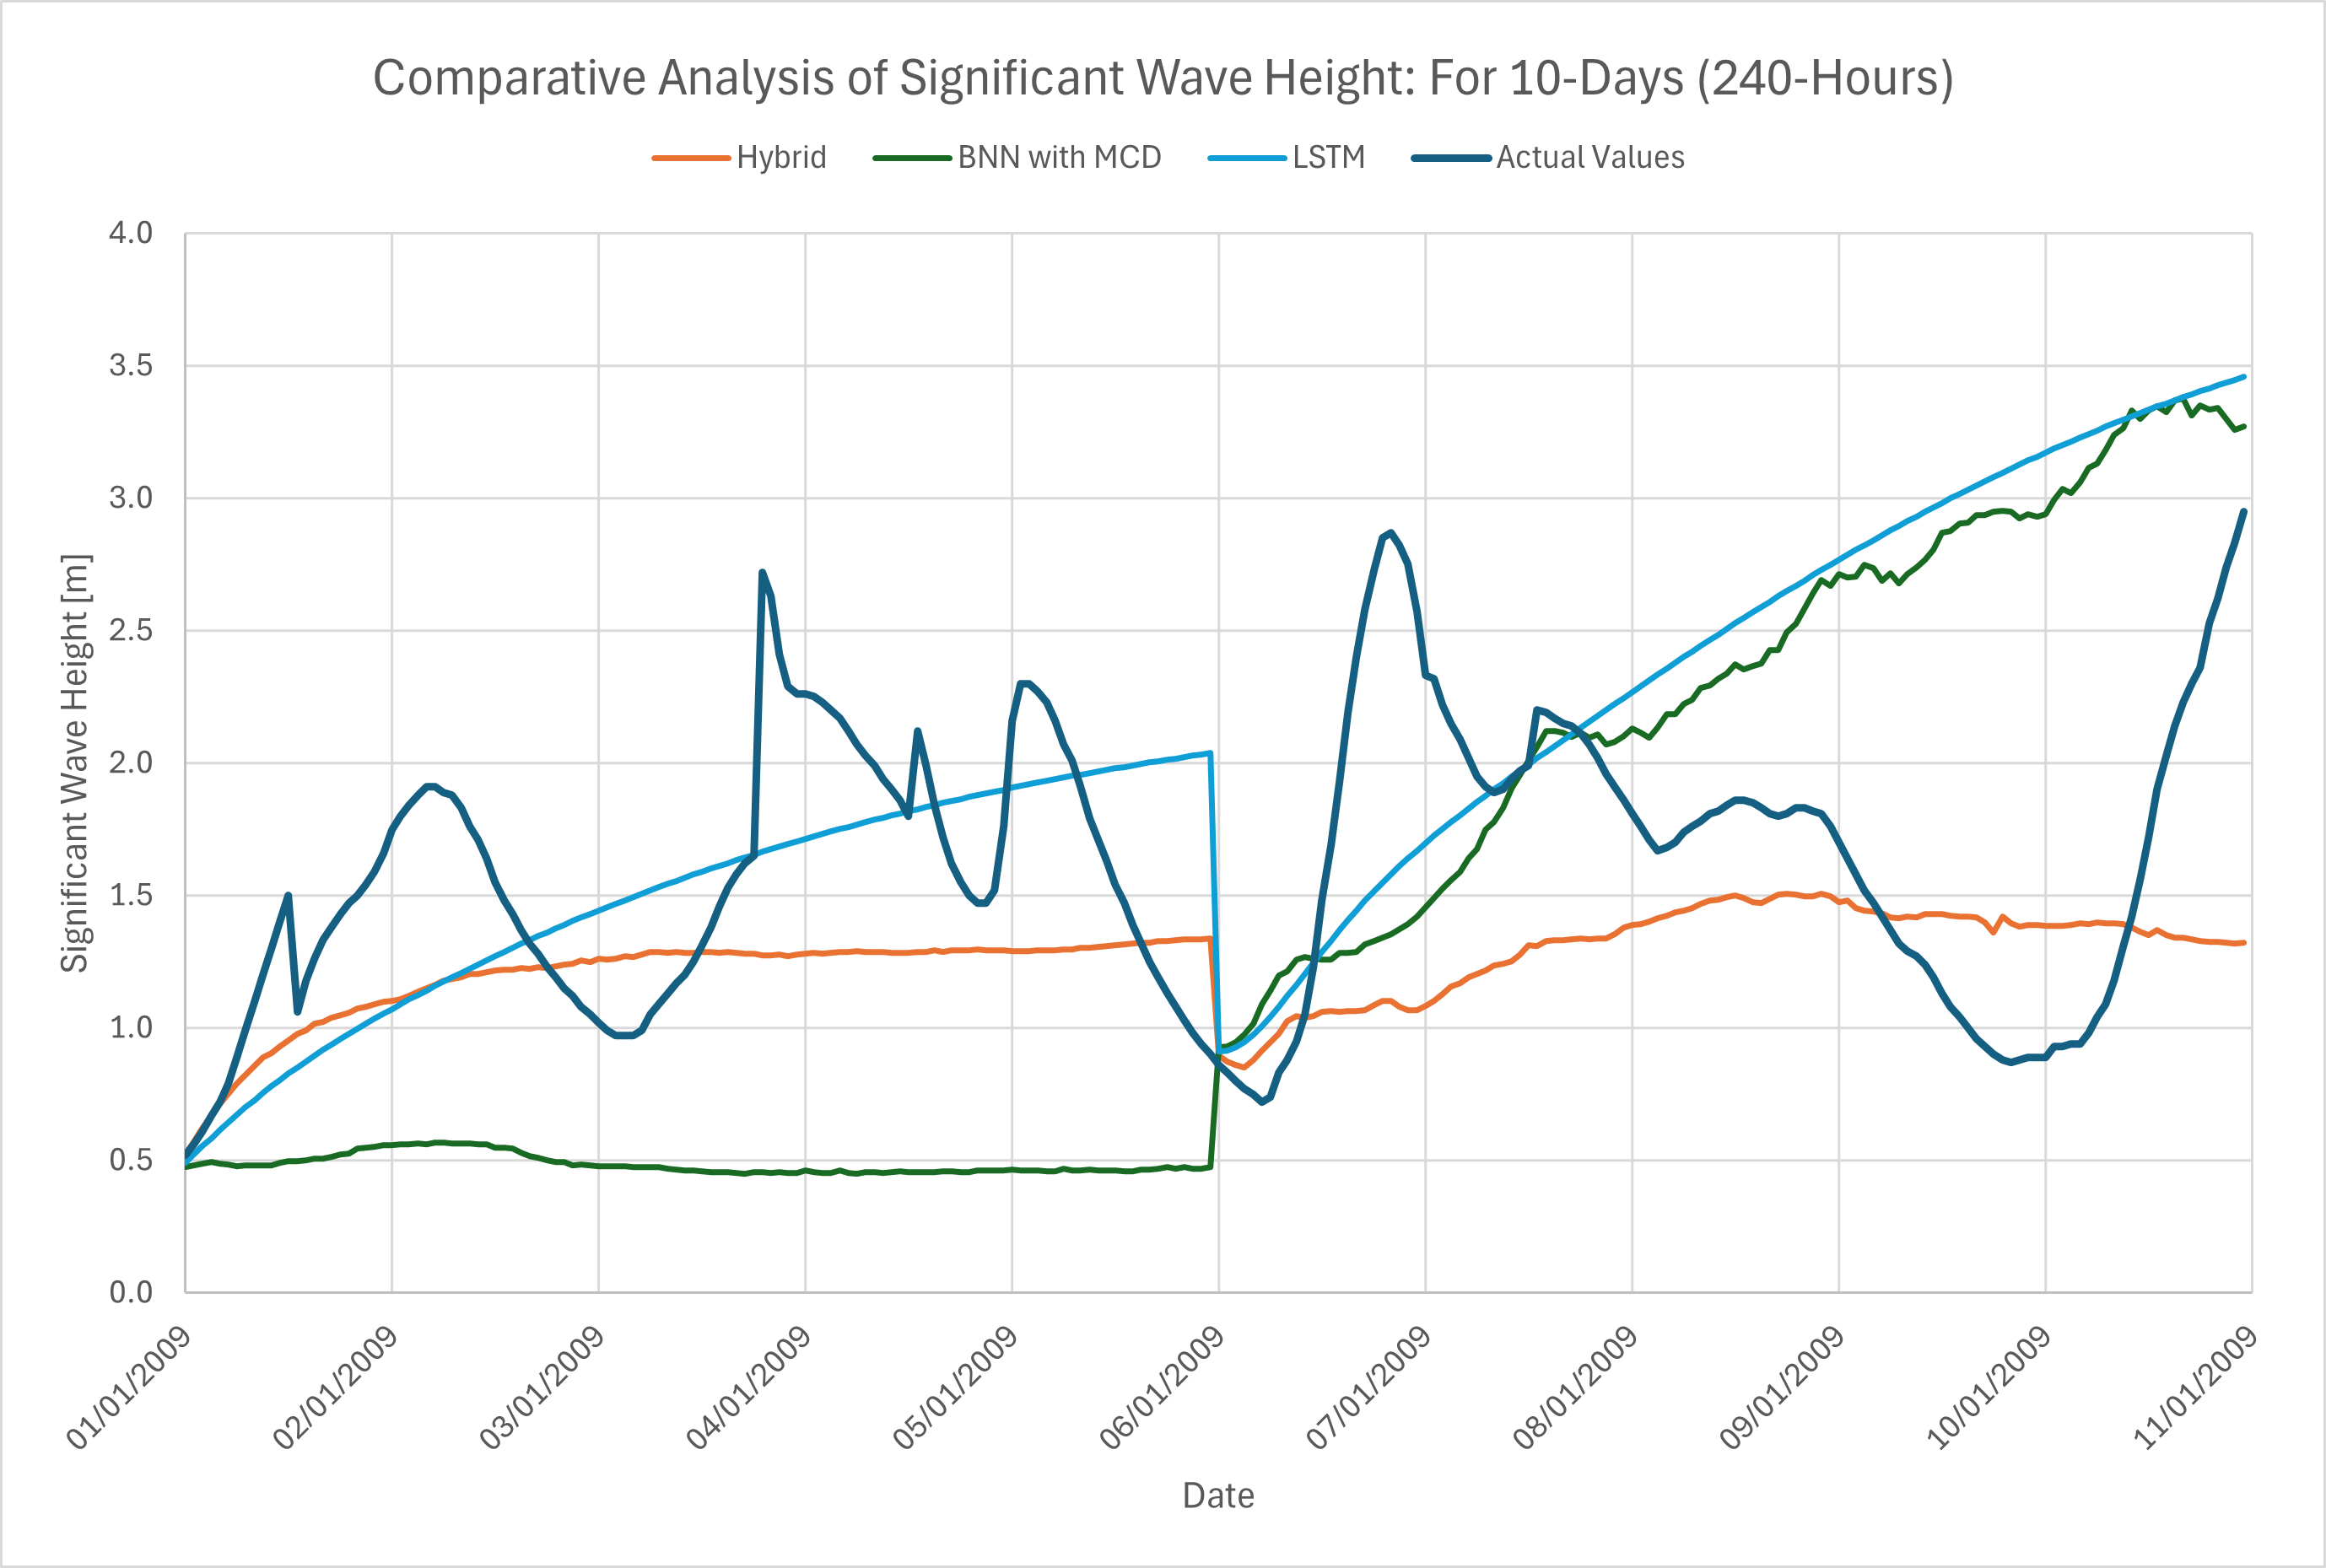
\includegraphics[width=\textwidth]{graphs/s_wht 240 hours.png}
        \caption{Significant Wave Height}
        \label{fig:s_wht_all_10Day}
    \end{subfigure}
    \hfill
    \begin{subfigure}[b]{0.49\textwidth}
        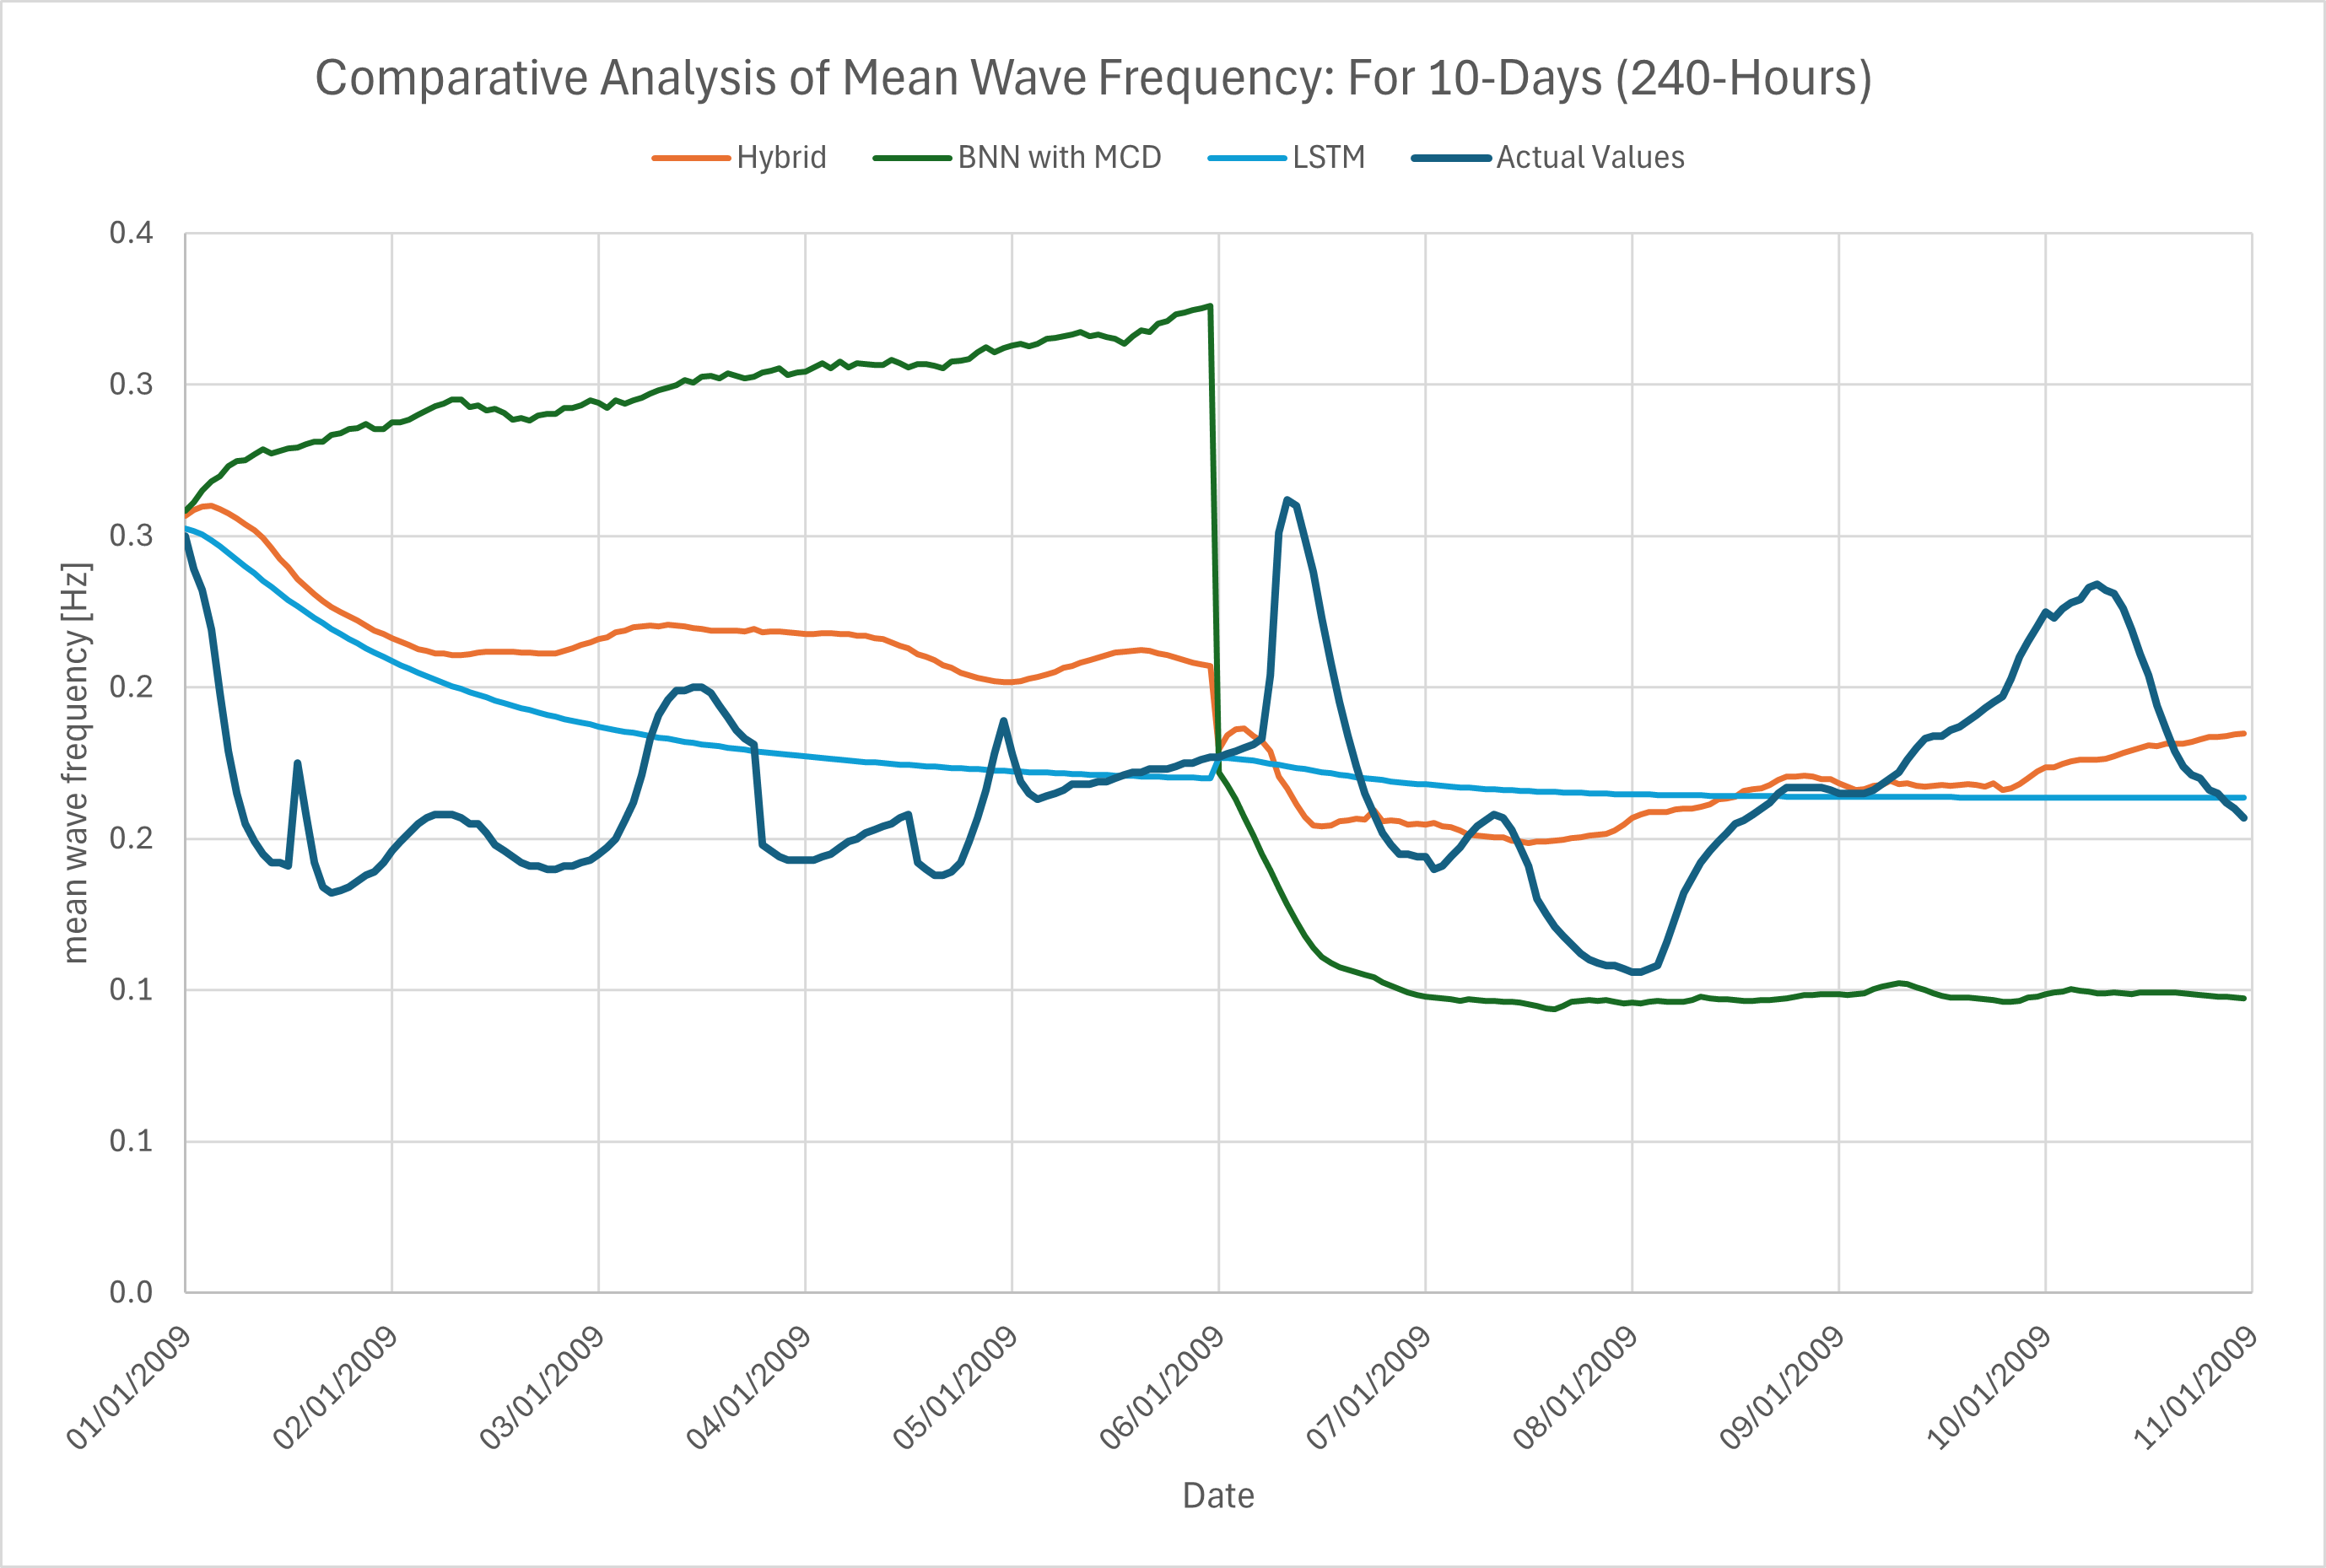
\includegraphics[width=\textwidth]{graphs/mean_fr 240 hours.png}
        \caption{Mean Wave Frequency}
        \label{fig:mean_fr_all_10Day}
    \end{subfigure}
    \vskip\baselineskip
    \begin{subfigure}[b]{0.49\textwidth}
        \centering
        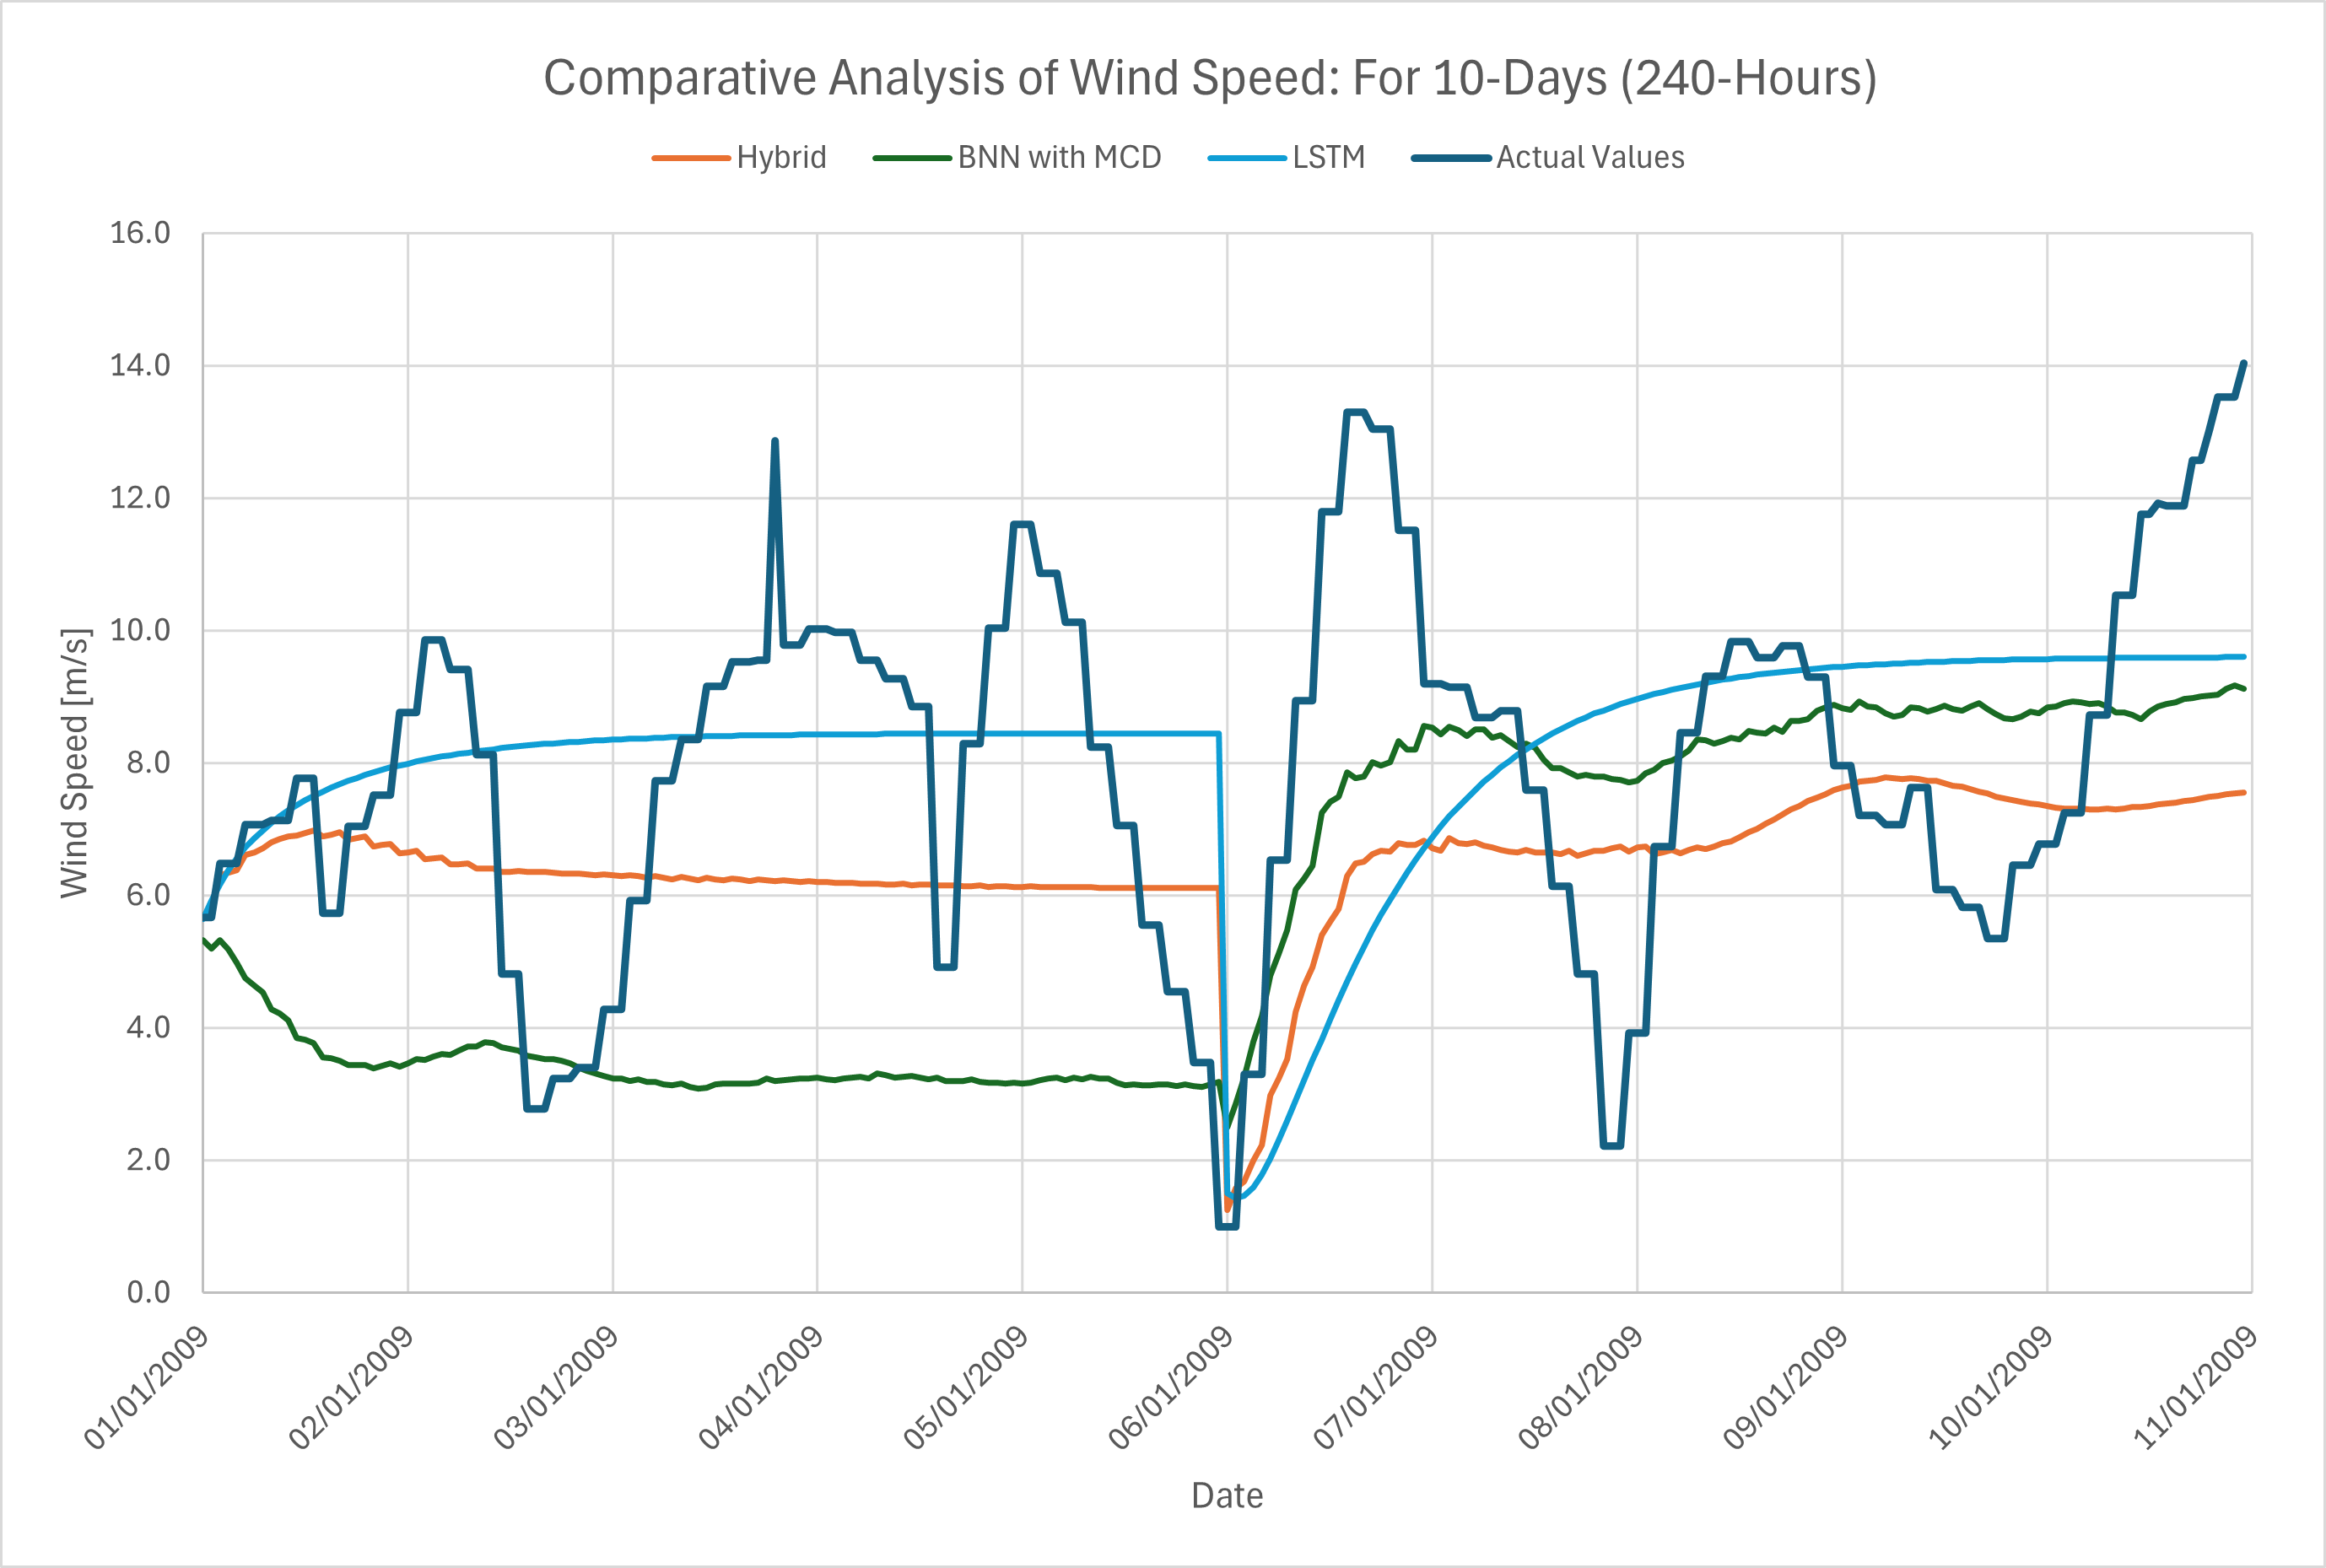
\includegraphics[width=\textwidth]{graphs/wind speed 240 hours.png}
        \caption{Wind Speed}
        \label{fig:wind_speed_all_10Day}
    \end{subfigure}
    \caption{Comparative analyses over the first 10 days (240 hours)}
    \label{fig:combined_10day}
\end{figure}

\noindent To estimate how well the models perform, the residuals are evaluated with a box plot in Figure \ref{fig:combined_box}. These plots show how the residuals of all forecasts are distributed to the actual values. Each box shows the interquartile range (IQR), the horizontal line inside the box is the median, the "x" symbol marks the mean. Whiskers extend to 1.5 times the IQR and individual residuals are shown outside the range.\\

\noindent The Hybrid model has distribution of the residuals that look stable. Although showing a median below zero, suggesting it is underfitting, the spread of the forecasted values is much lower. If looking at the BNN with MCD, the spread in the residuals is much larger, which indicates there is more variability between the residuals. This is not beneficial where the forecast accuracy will go down when this residual spread is higher. The residuals of the LSTM model show somewhat the same range, but there is one significant difference in the outliers. This model has a lot of outliers above the Whisker extend, suggesting there are a lot of forecasted values above the actual values.\\

\begin{figure}[ht!]
    \centering
    \begin{subfigure}[b]{0.49\textwidth}
        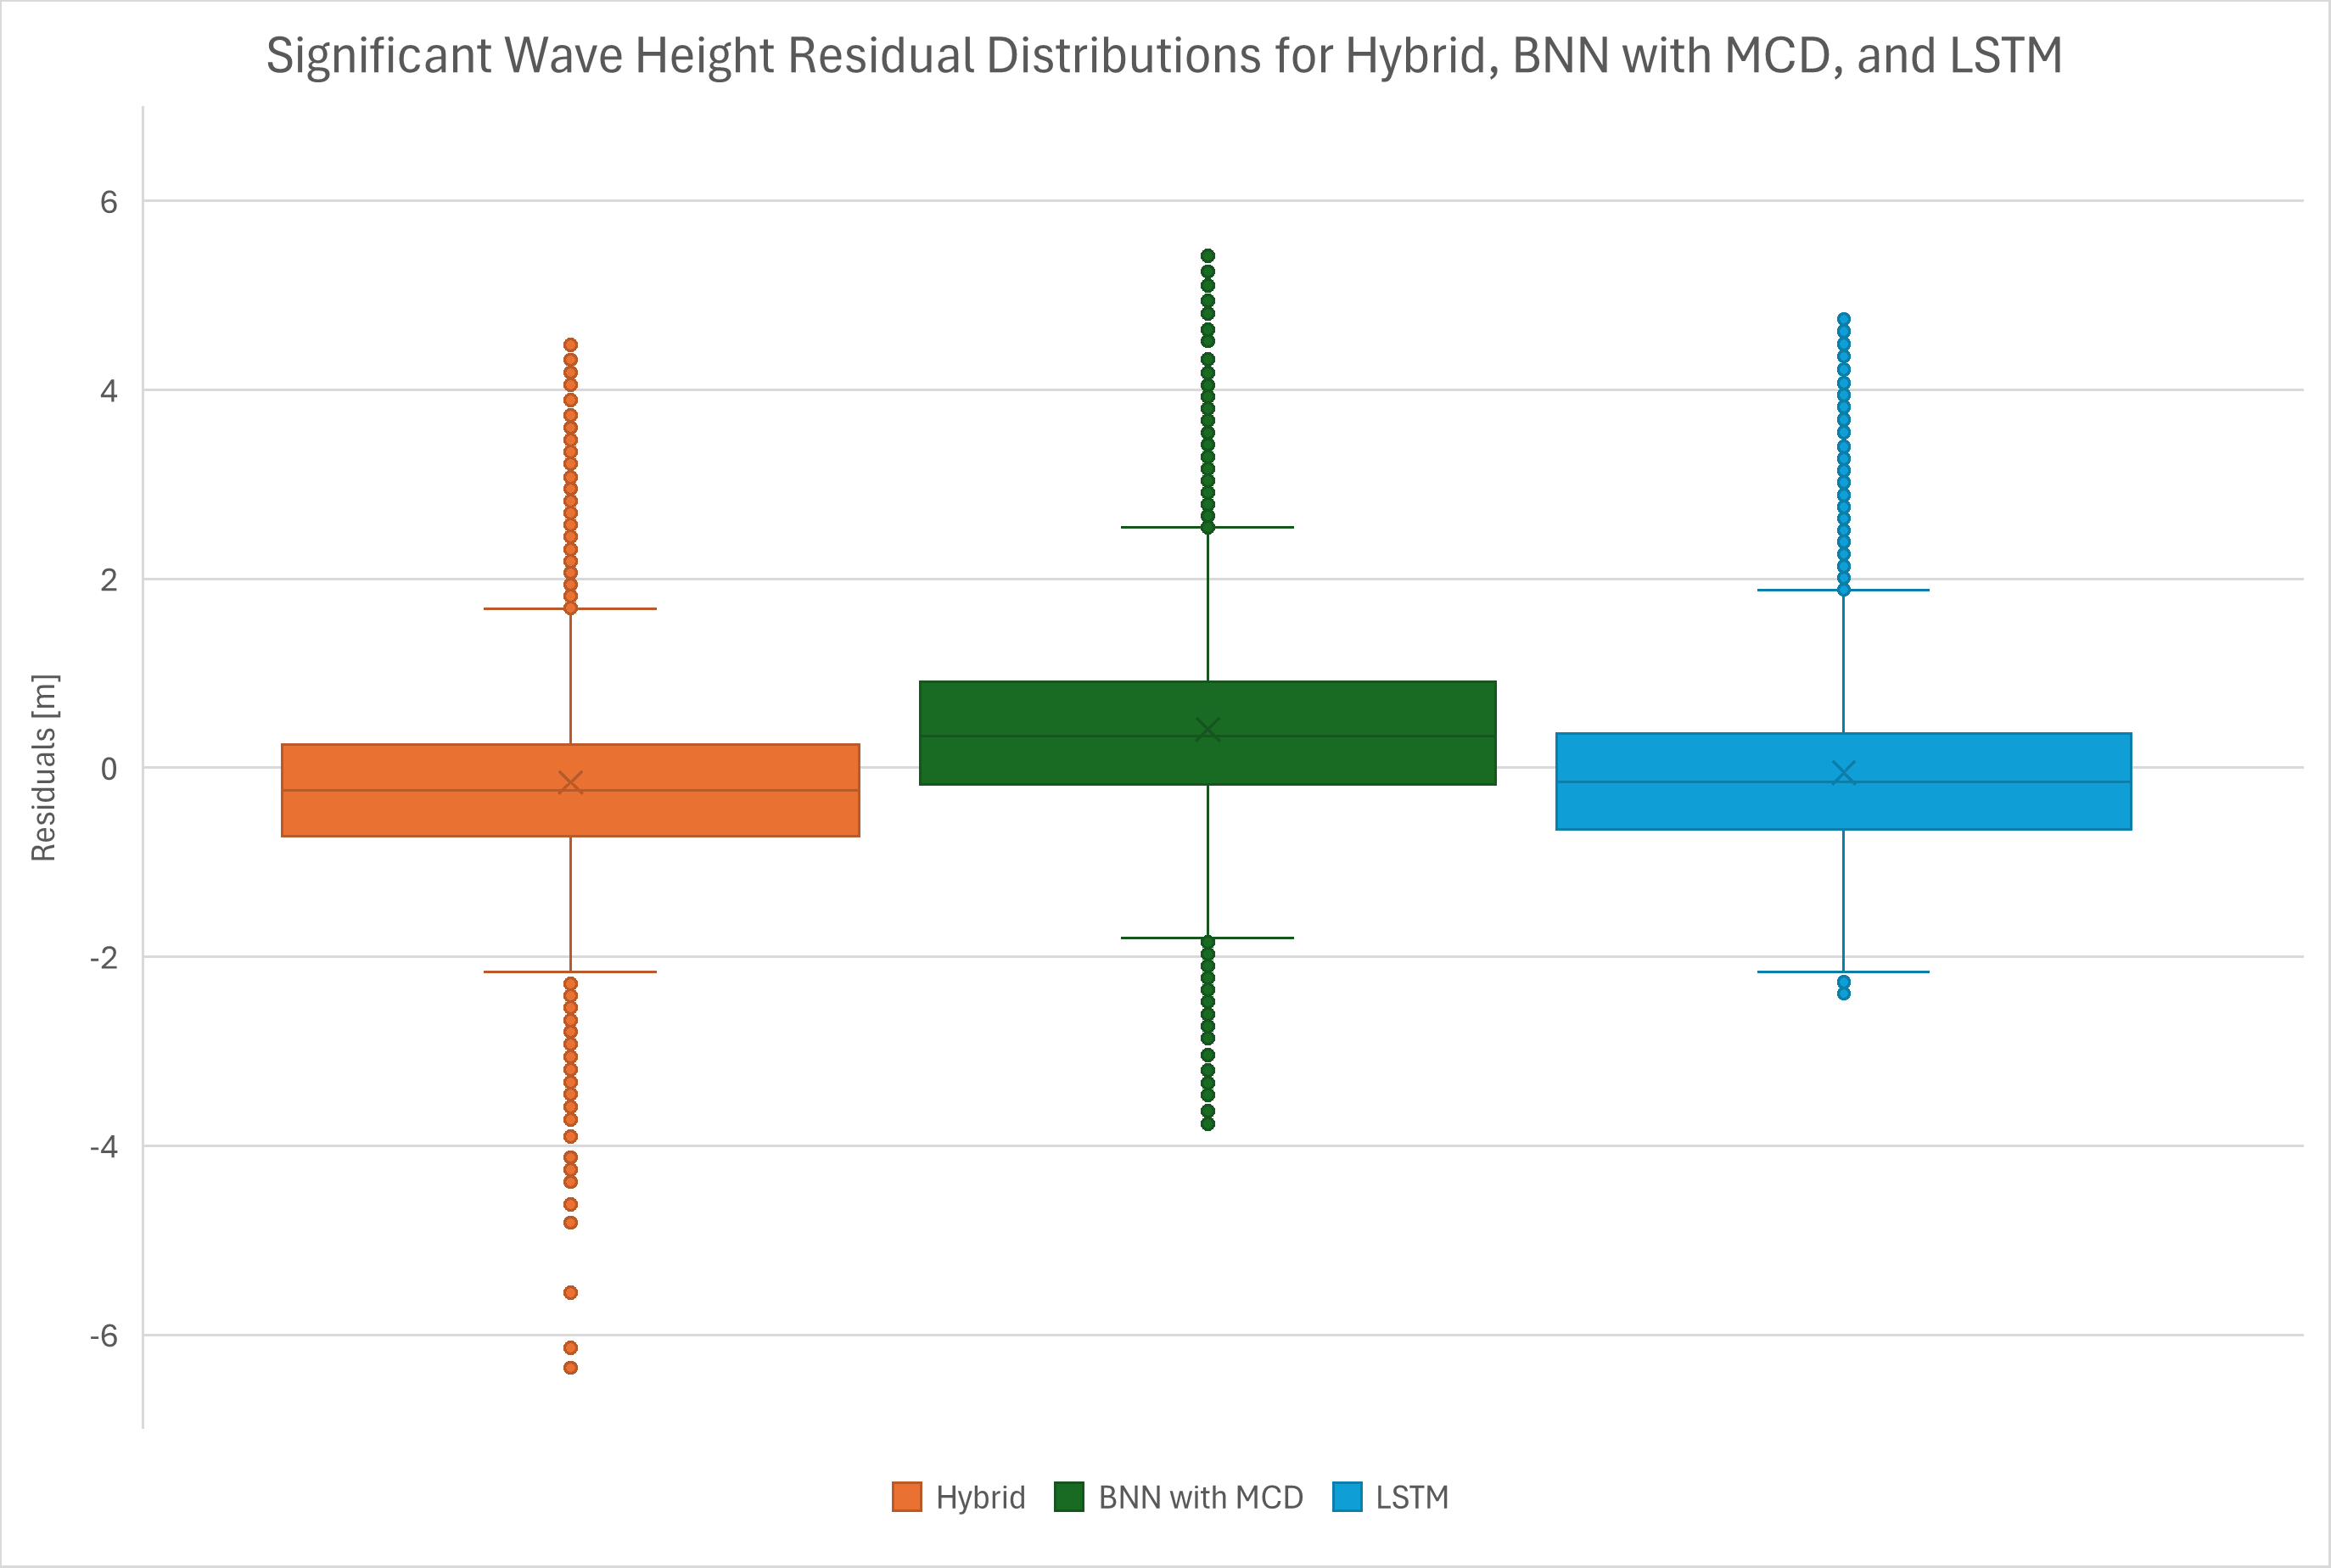
\includegraphics[width=\textwidth]{graphs/Box s_wht.png}
        \caption{Significant Wave Height}
        \label{fig:s_wht_box}
    \end{subfigure}
    \hfill
    \begin{subfigure}[b]{0.49\textwidth}
        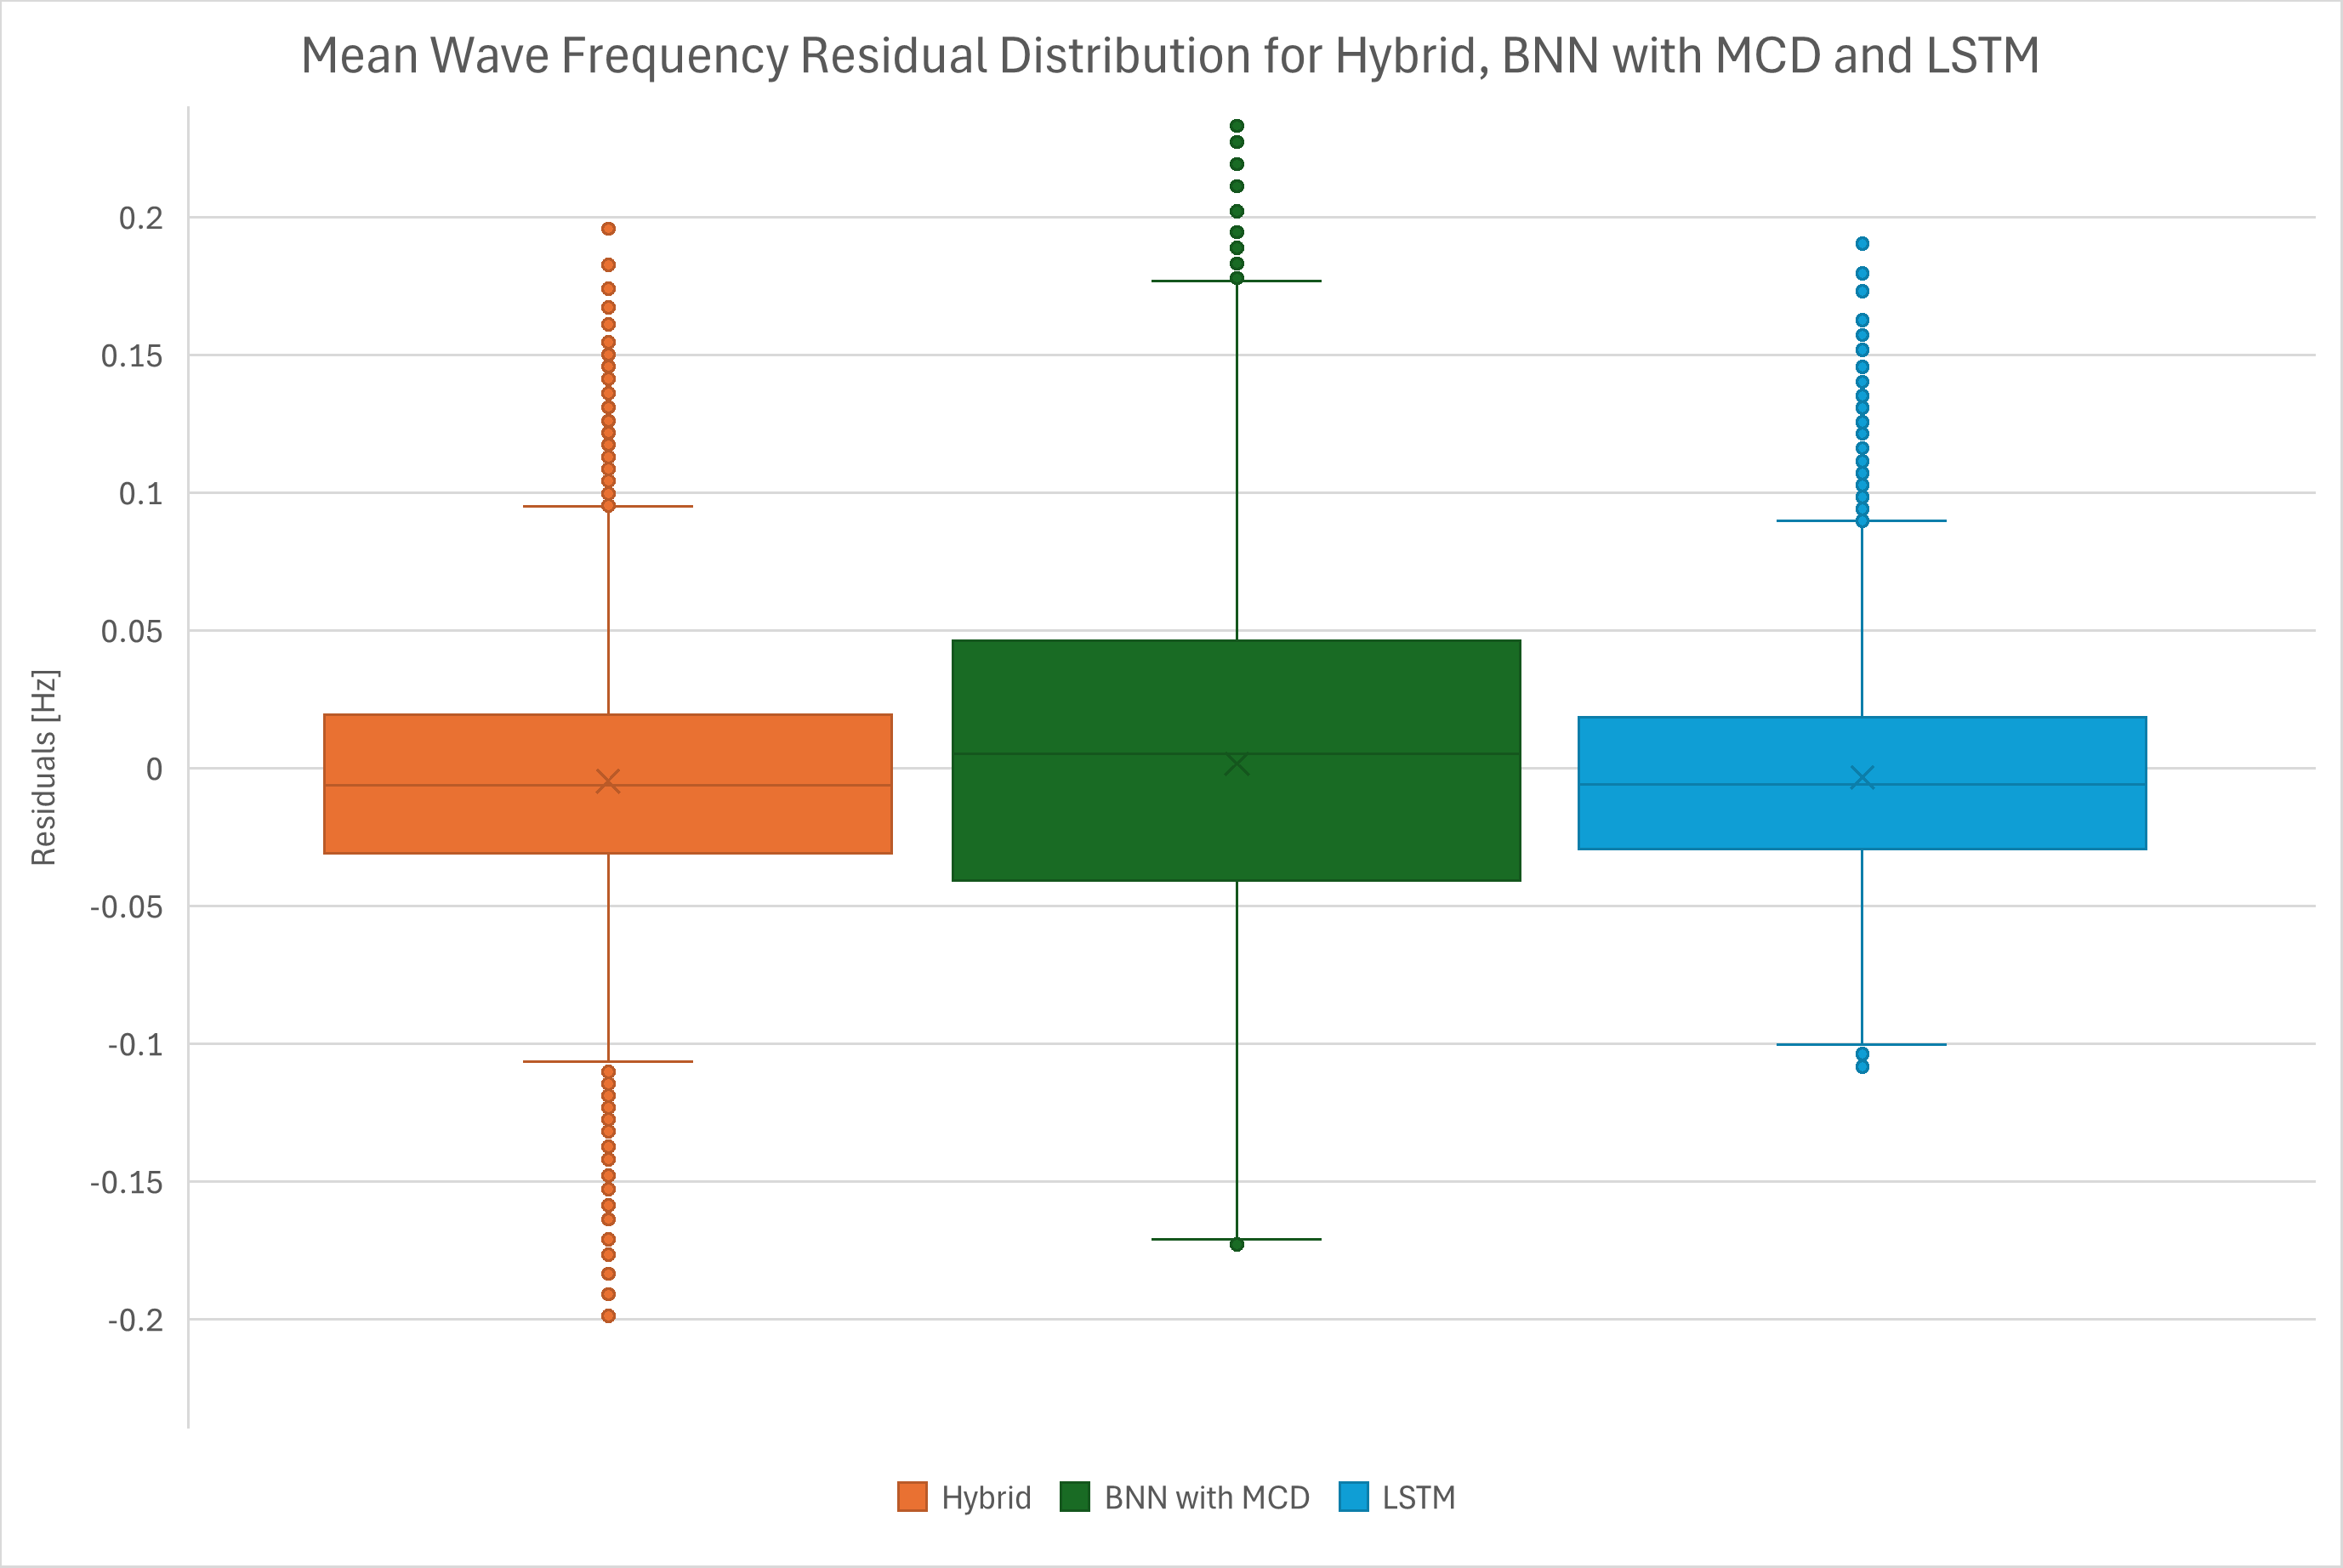
\includegraphics[width=\textwidth]{graphs/Box mean_fr.png}
        \caption{Mean Wave Frequency}
        \label{fig:mean_fr_box}
    \end{subfigure}
    \vskip\baselineskip
    \begin{subfigure}[b]{0.49\textwidth}
        \centering
        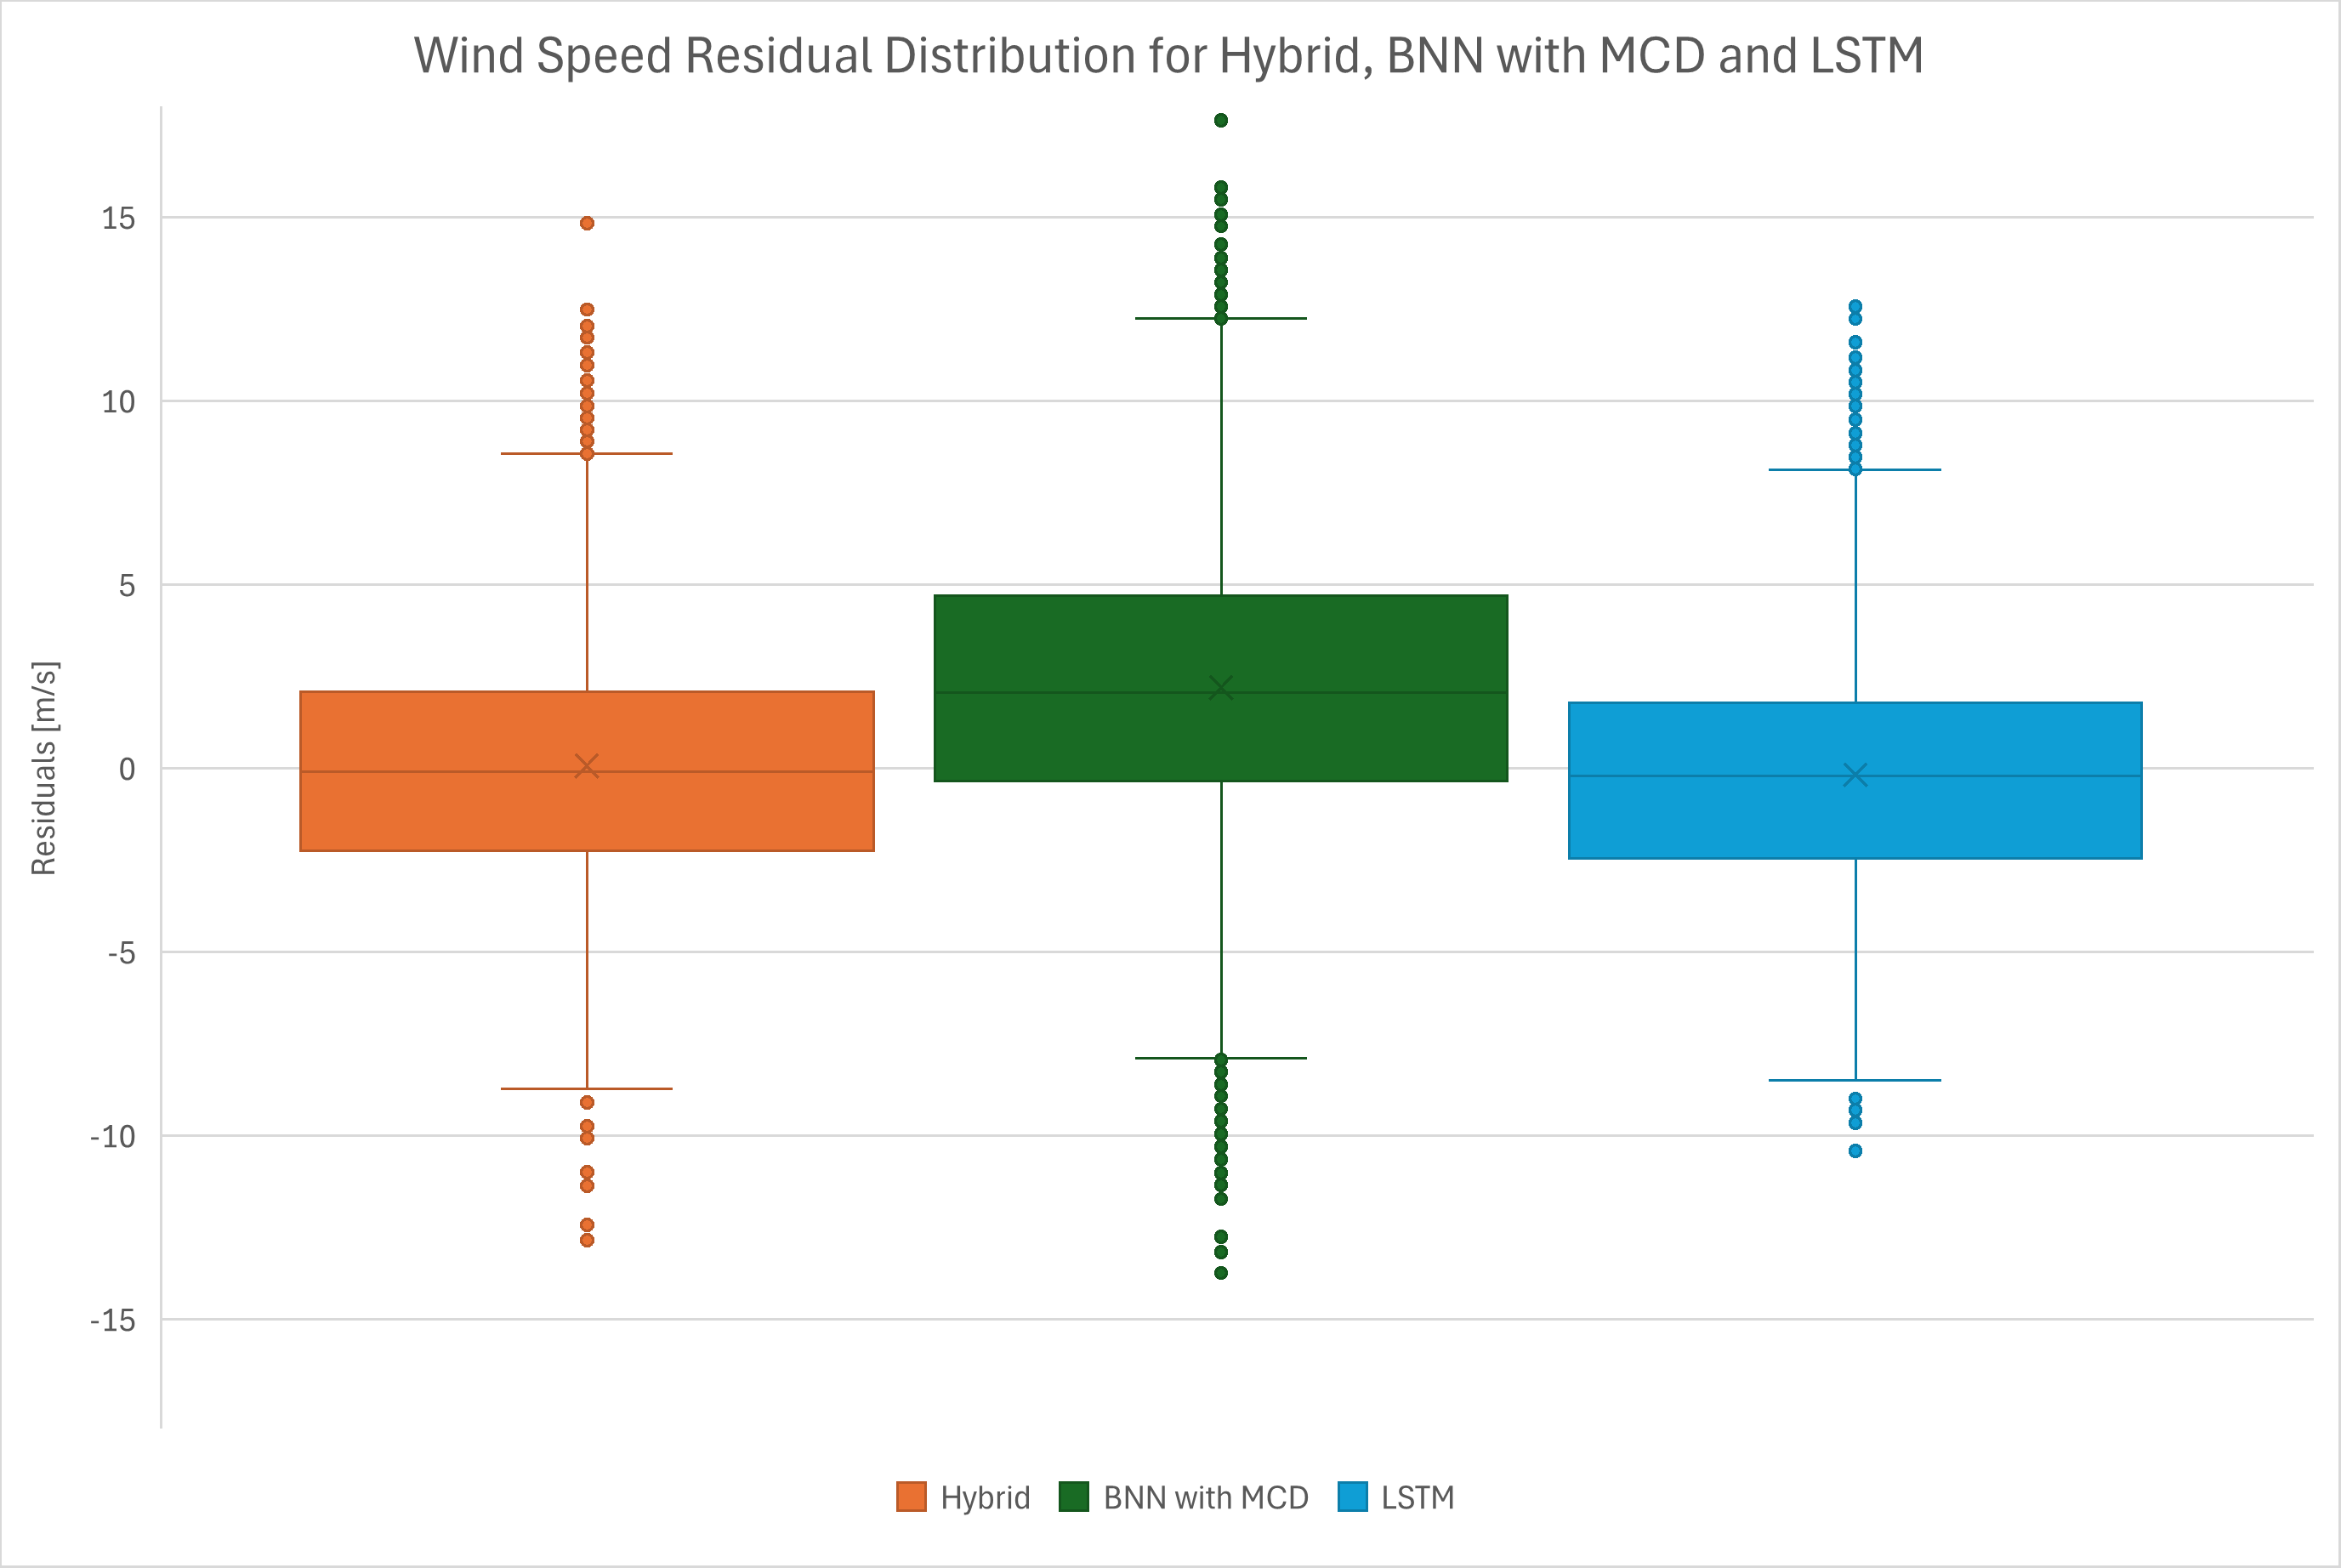
\includegraphics[width=\textwidth]{graphs/Box wind_speed.png}
        \caption{Wind Speed}
        \label{fig:wind_speed_box}
    \end{subfigure}
    \caption{Comparative box plot of significant wave height, mean wave frequency, and wind speed}
    \label{fig:combined_box}
\end{figure}

\noindent Overall, the comparative results indicate the three models are capturing the overall trends; how they do so differs a lot. The forecasted values plotted against the actual values, the residuals plot and a scatter plot of each model can be found in Appendix \ref{results all models 5 days}. The LSTM model shows exponential tendencies as visible in Figure \ref{fig:s_wht_all_10Day}. The BNN with MCD shows greater variability in the box plots, which is not beneficial when an accurate forecast is necessary. The Hybrid model shows consistent forecasts with a low error and its residuals tend to stay closer to the mean. These reasons to further analyse the Hybrid ARIMA-ANN model.

\newpage

\section{Hybrid Model Results}
\label{hybrid_model_results}
This section will investigate the sensitivity of the Hybrid model with the usage of different refit intervals, these are: 6 hours, 12 hours, 1 day, 2 days, 3 days, 4 days, 5 days, 6 days, 7 days, 2 weeks, 4 weeks. The forecasted values against the actual values, the residuals plot and the scatter plots for each refit interval can be seen in Appendix \ref{results hybrid different refit}.\\

\noindent While there are a lot of different outcomes for the evaluation metrics: MSE, MAE, RMSE and $R^2$ will be evaluated with the graphs in Figure \ref{fig:hybrid_refit_metrics}. The left y-axis is used for the MSE, MAE and RMSE, and the right y-axis showcases the $R^2$ values. The x-axis is not equally weighted, so the distance between 0.25 and 0.5 days is the same as the distance between 7 days and 14 days. For the significant wave height in Figure \ref{fig:s_wht_refit} and the mean wave frequency in Figure \ref{fig:mean_fr_refit}, it can be seen that the curves steadily increase for the MSE, MAE, and RMSE over time. Another thing visible is that around the 3-day refit interval rate the $R^2$ drops below zero, indicating the model is outperformed by a naive baseline. For the wind speed in Figure \ref{fig:wind_speed_refit} the errors increase much less drastically and seem to move towards a maximum value over time. Also, the $R^2$ only drops below zero after around a 5 day interval, all indicating the model performs best on this parameter. Overall longer refit intervals lead to higher values of MSE, MAE and RMSE and lower values for $R^2$

\begin{figure}[ht!]
    \centering
    \begin{subfigure}[b]{0.49\textwidth}
        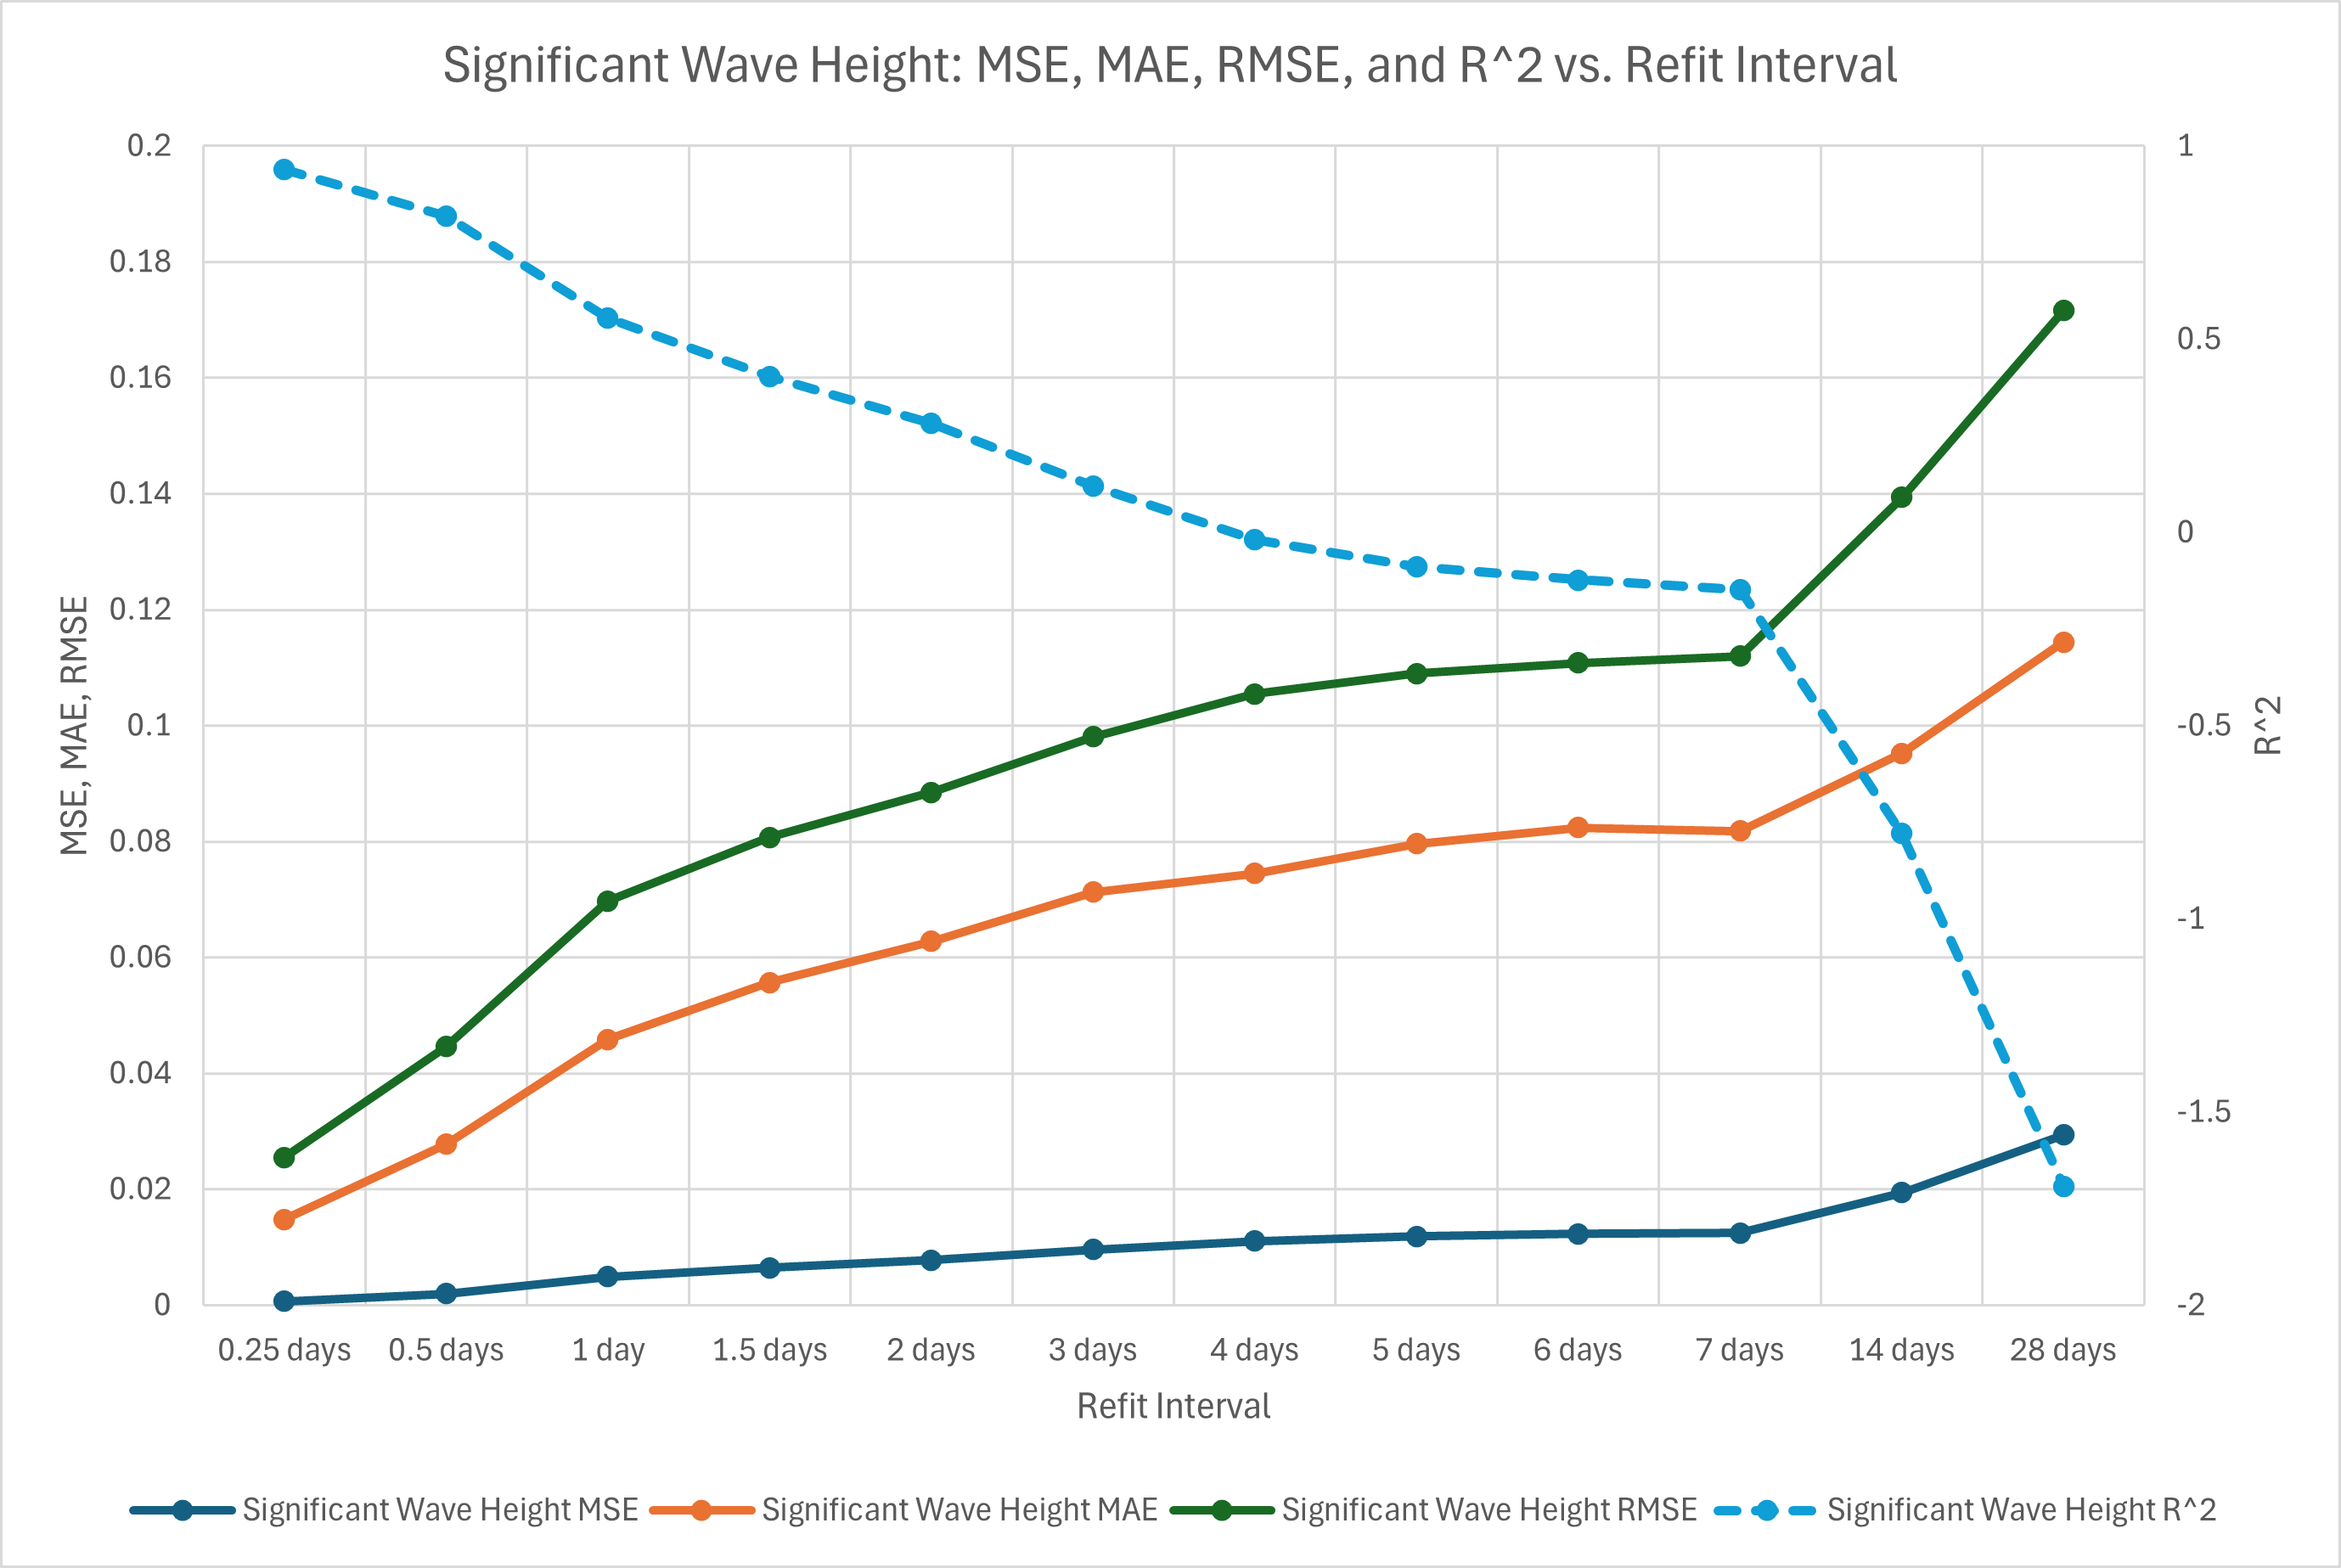
\includegraphics[width=\textwidth]{graphs/Refit_s_wht_metrics.png}
        \caption{Significant Wave Height}
        \label{fig:s_wht_refit}
    \end{subfigure}
    \hfill
    \begin{subfigure}[b]{0.49\textwidth}
        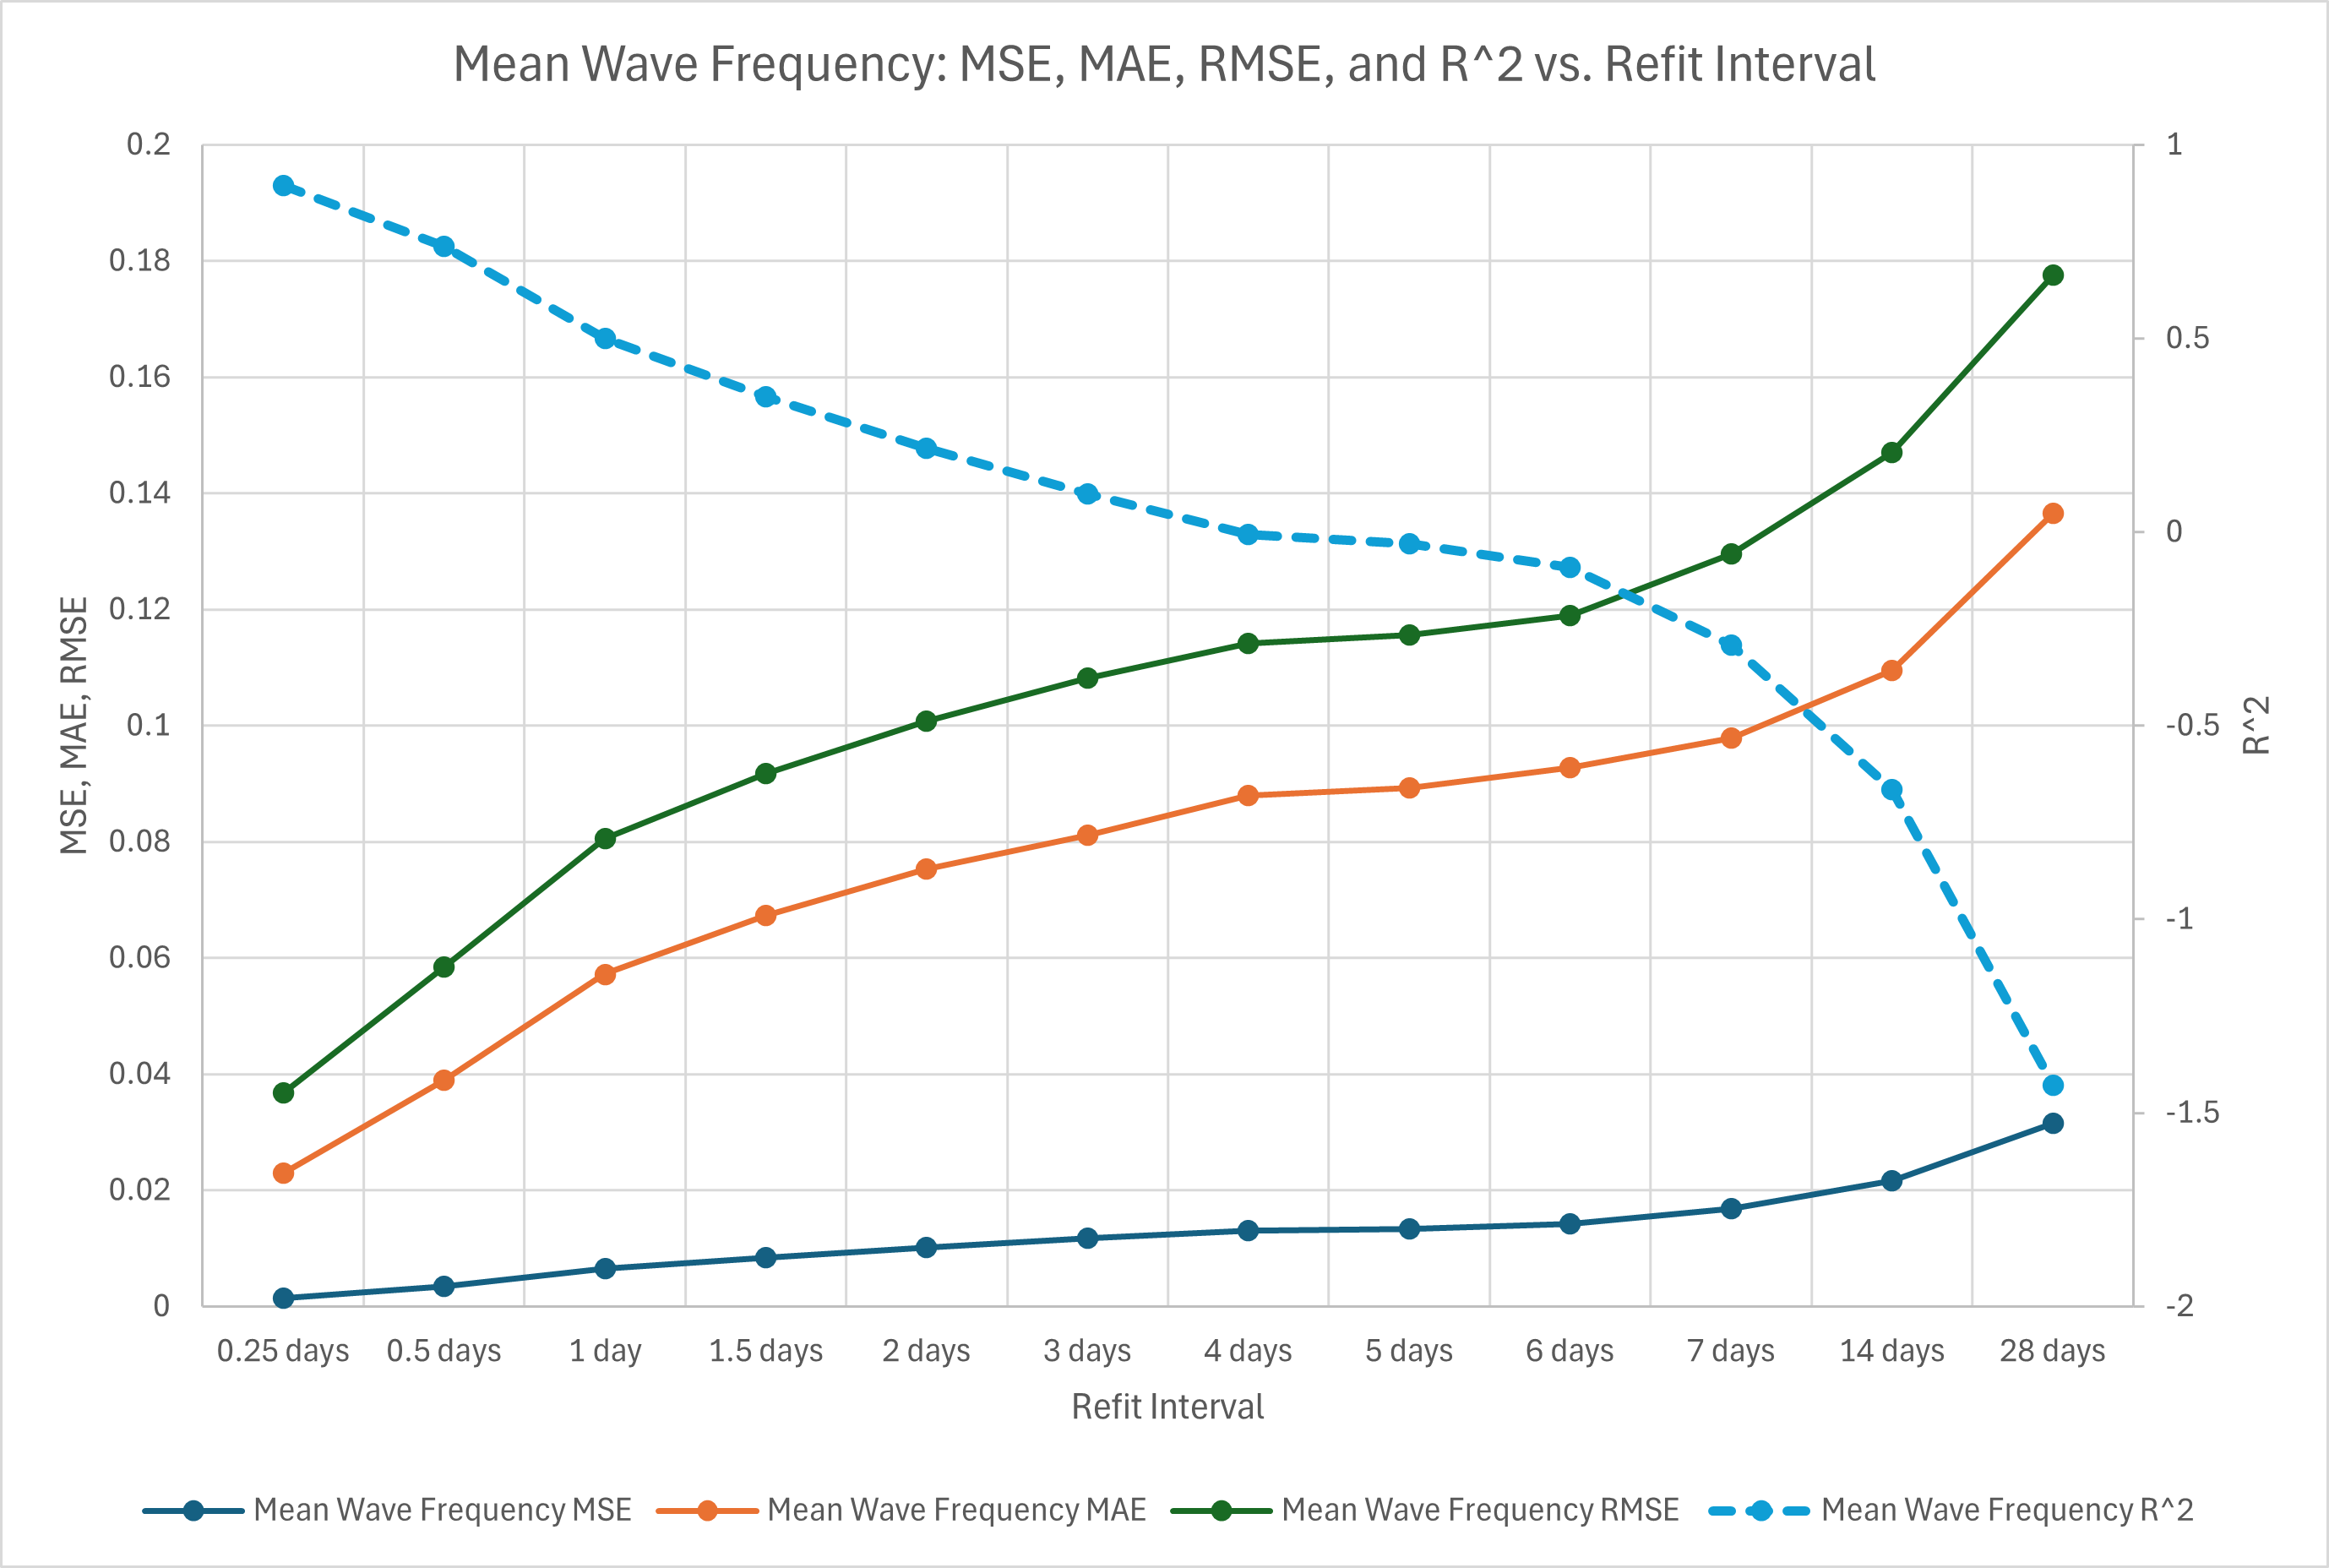
\includegraphics[width=\textwidth]{graphs/Refit_mean_fr_metrics.png}
        \caption{Mean Wave Frequency}
        \label{fig:mean_fr_refit}
    \end{subfigure}
    \vskip\baselineskip
    \begin{subfigure}[b]{0.49\textwidth}
        \centering
        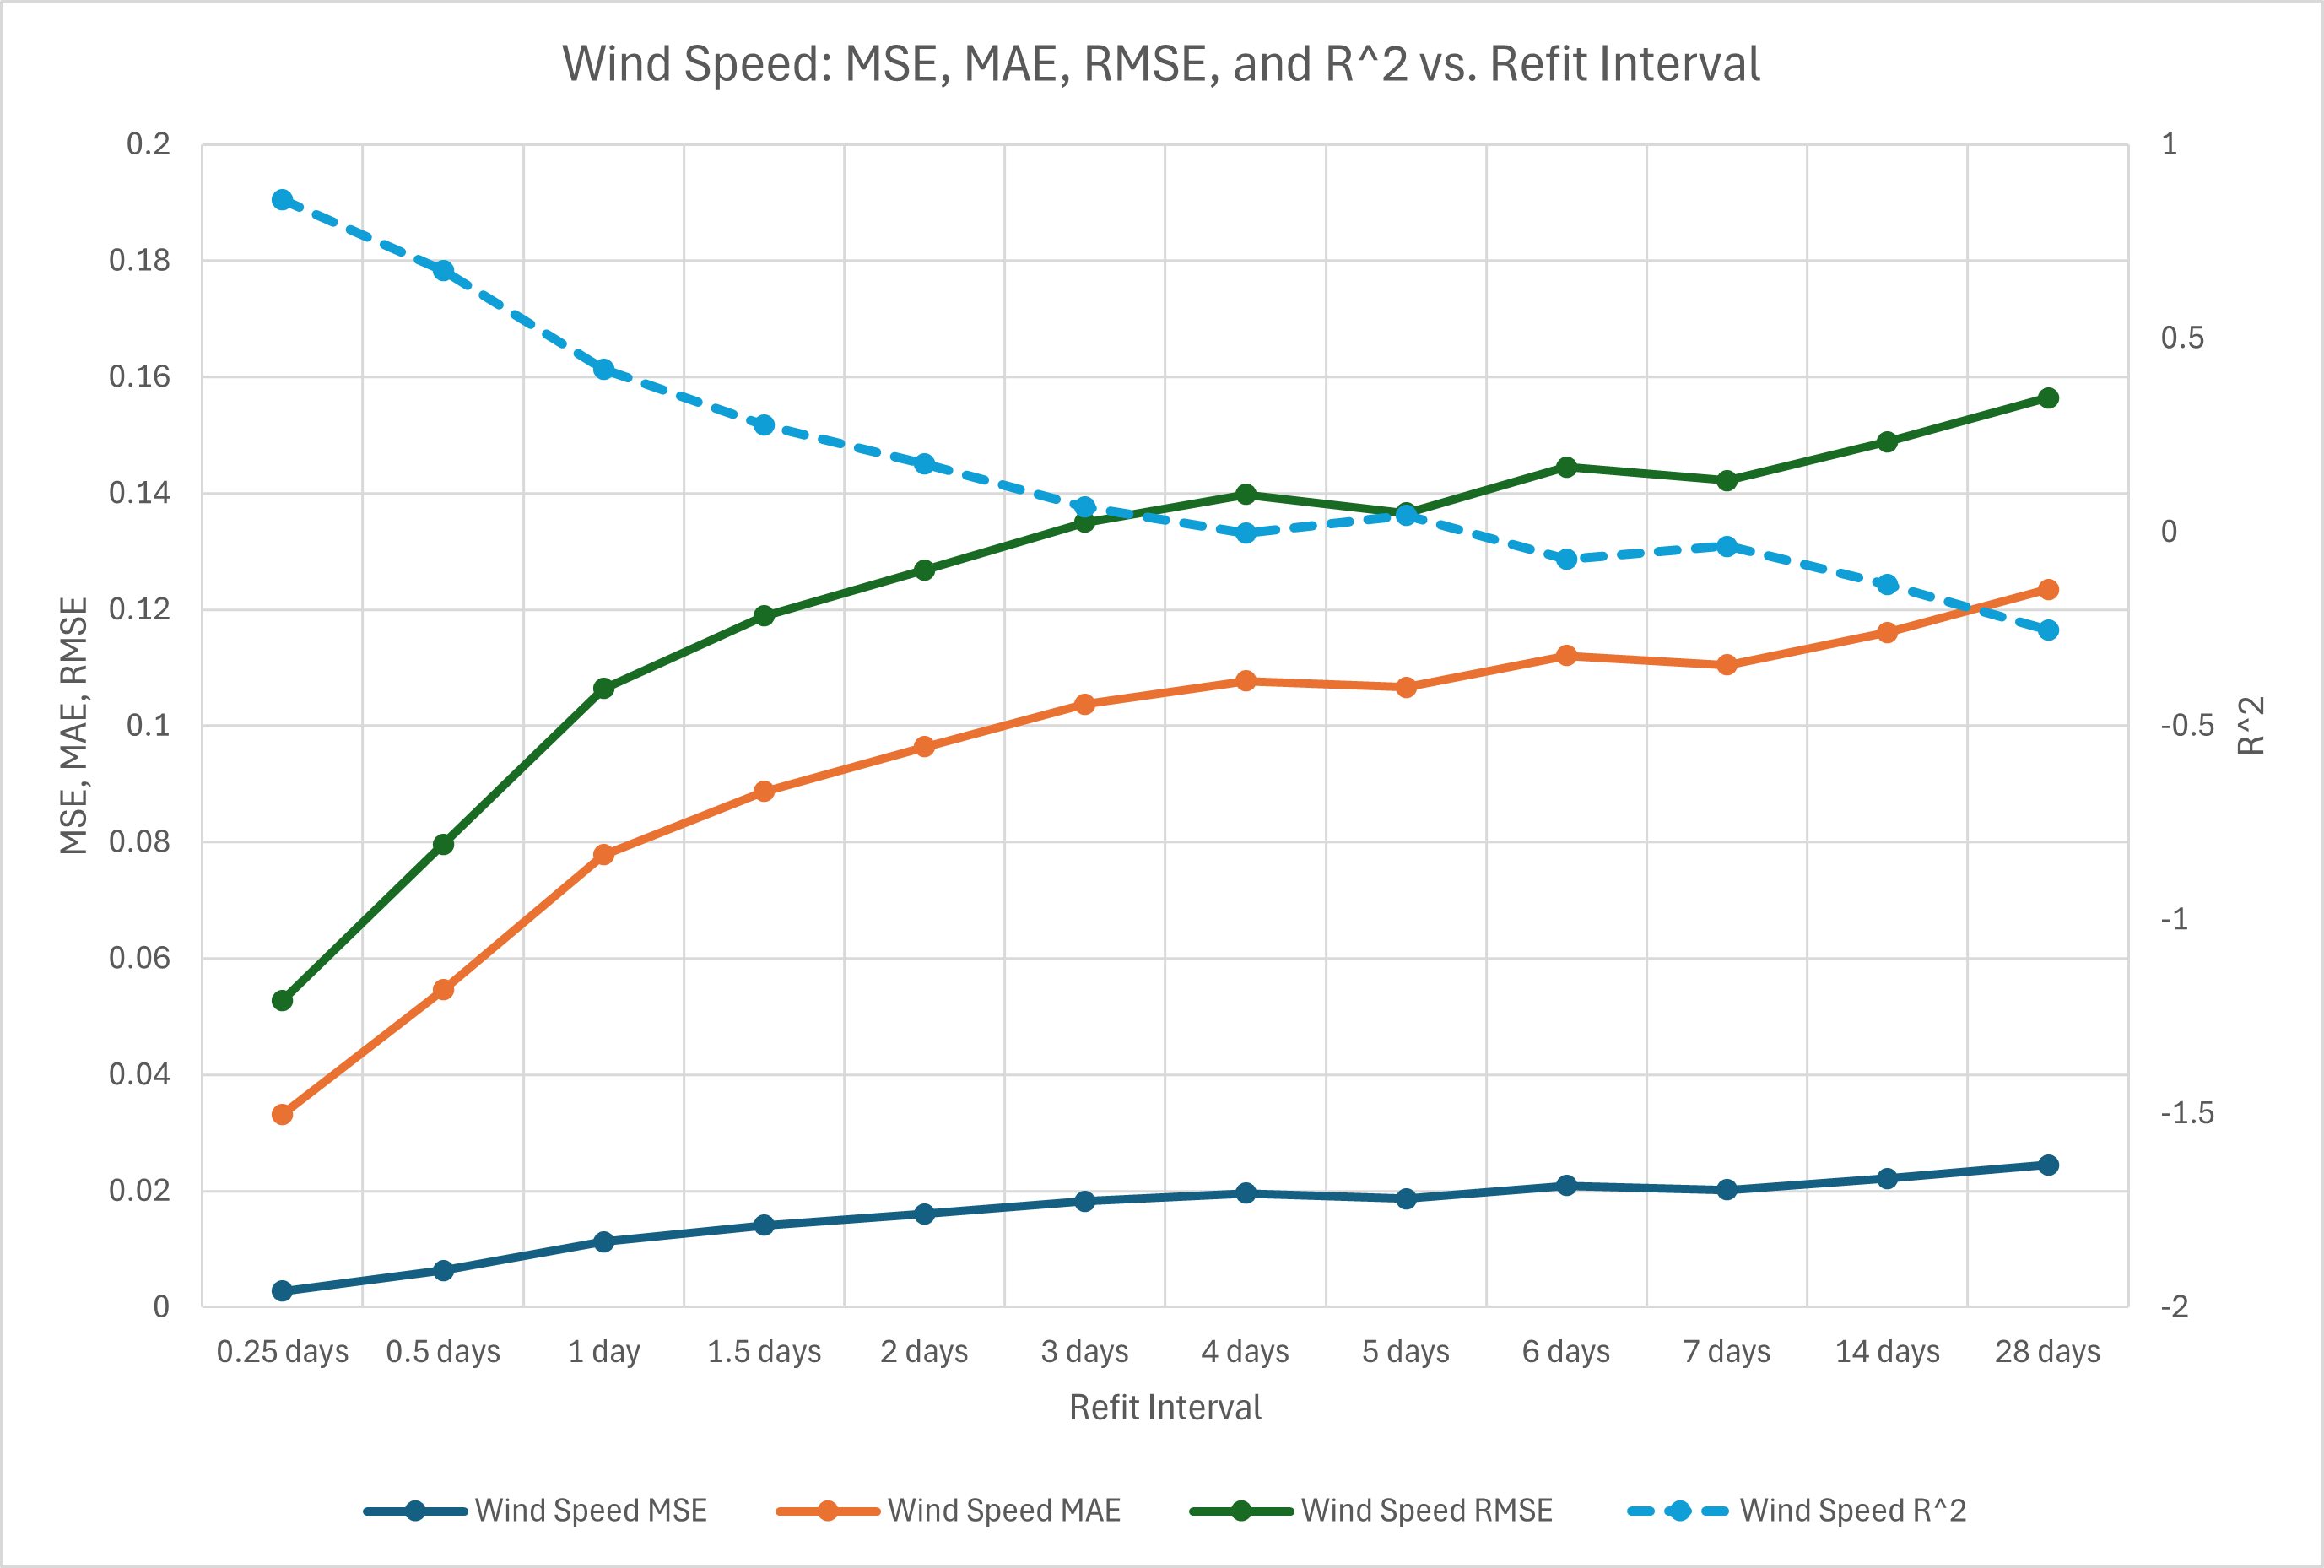
\includegraphics[width=\textwidth]{graphs/Refit_wind_speed_metrics.png}
        \caption{Wind Speed}
        \label{fig:wind_speed_refit}
    \end{subfigure}
    \caption{Line Plots of the Hybrid ARIMA–ANN model’s performance metrics ( MSE, MAE, RMSE, $R^{2}$) under varying refit intervals.}
    \label{fig:hybrid_refit_metrics}
\end{figure}

\newpage

\noindent Below in Figure \ref{fig:hybrid_refit_box}, each box presents the distribution of the residuals for each refit interval in the same way as in Figure \ref{fig:combined_box}. Again it is visible that a longer refit interval leads for all parameters to a larger deviation in the residual errors. The median and mean are in all cases around zero, which indicates the model has the error on average around zero. The model shows, for larger refit intervals, more residuals which fall outside the Whiskers extend. Especially for the values below zero, it is visible that there is a larger error, this indicates that the forecasted value is much larger than the actual value. 

\begin{figure}[ht!]
    \centering
    \begin{subfigure}[b]{0.49\textwidth}
        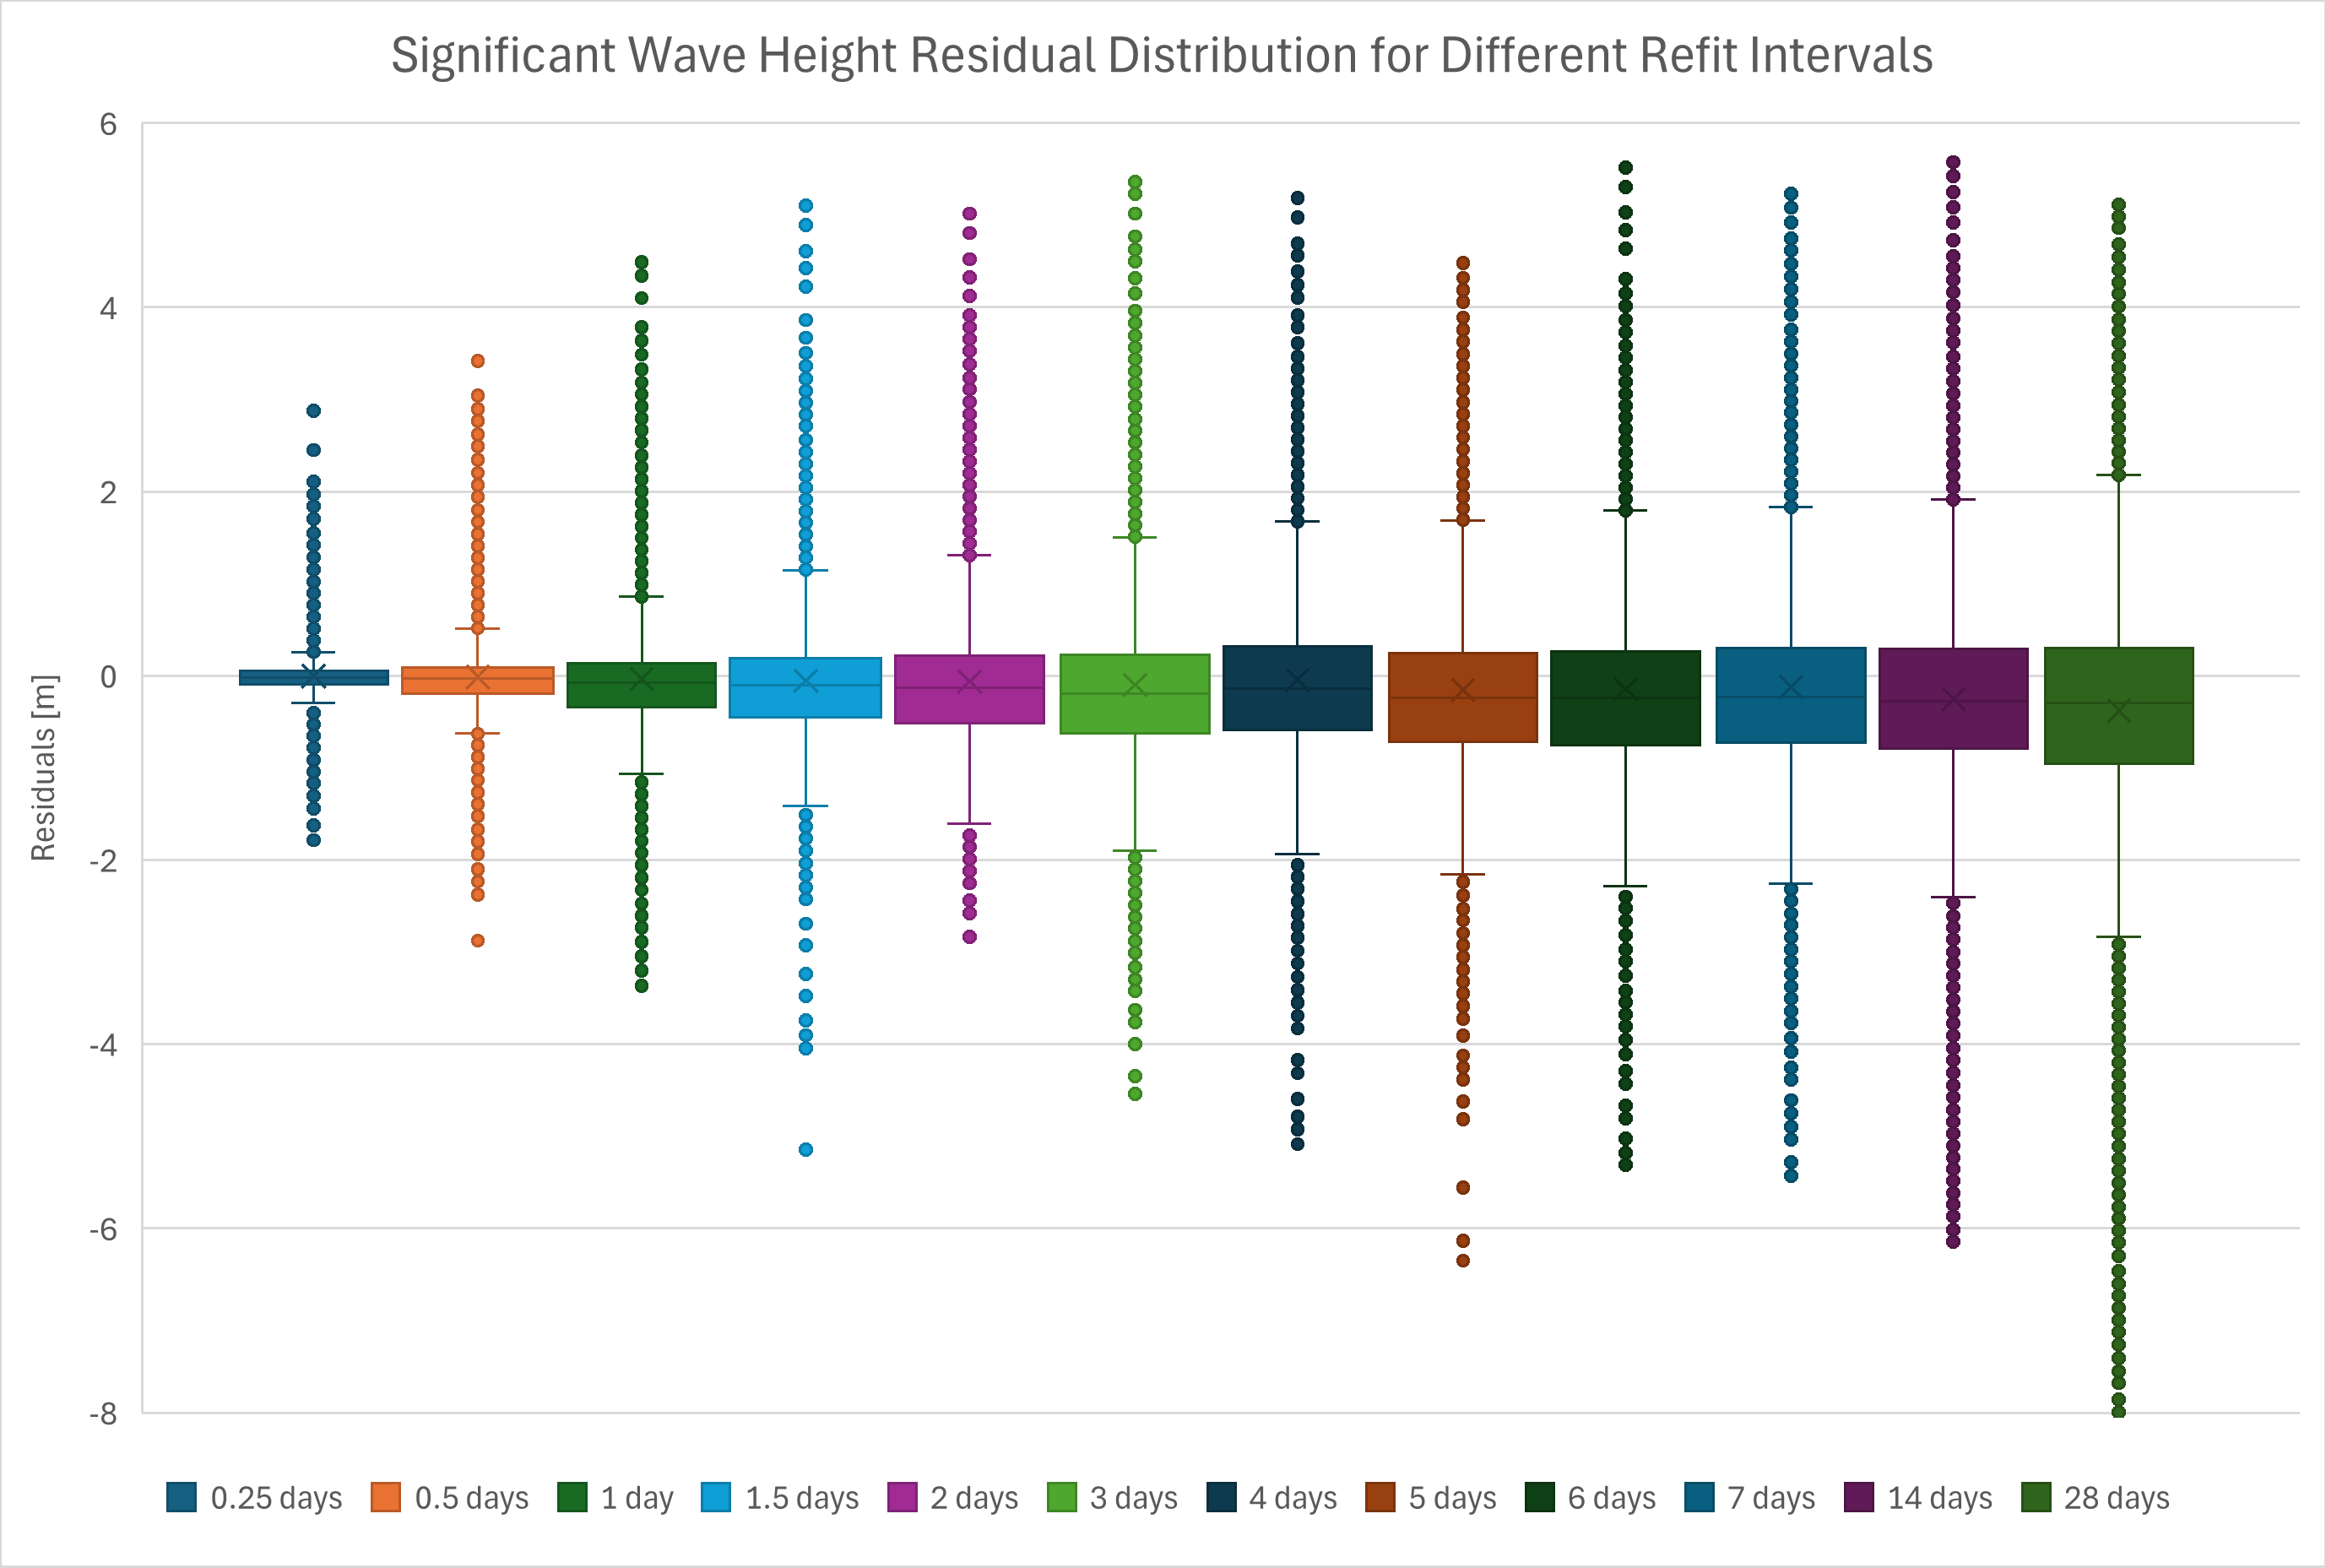
\includegraphics[width=\textwidth]{graphs/Box_refit_swht.png}
        \caption{Significant Wave Height}
        \label{fig:s_wht_refit_box}
    \end{subfigure}
    \hfill
    \begin{subfigure}[b]{0.49\textwidth}
        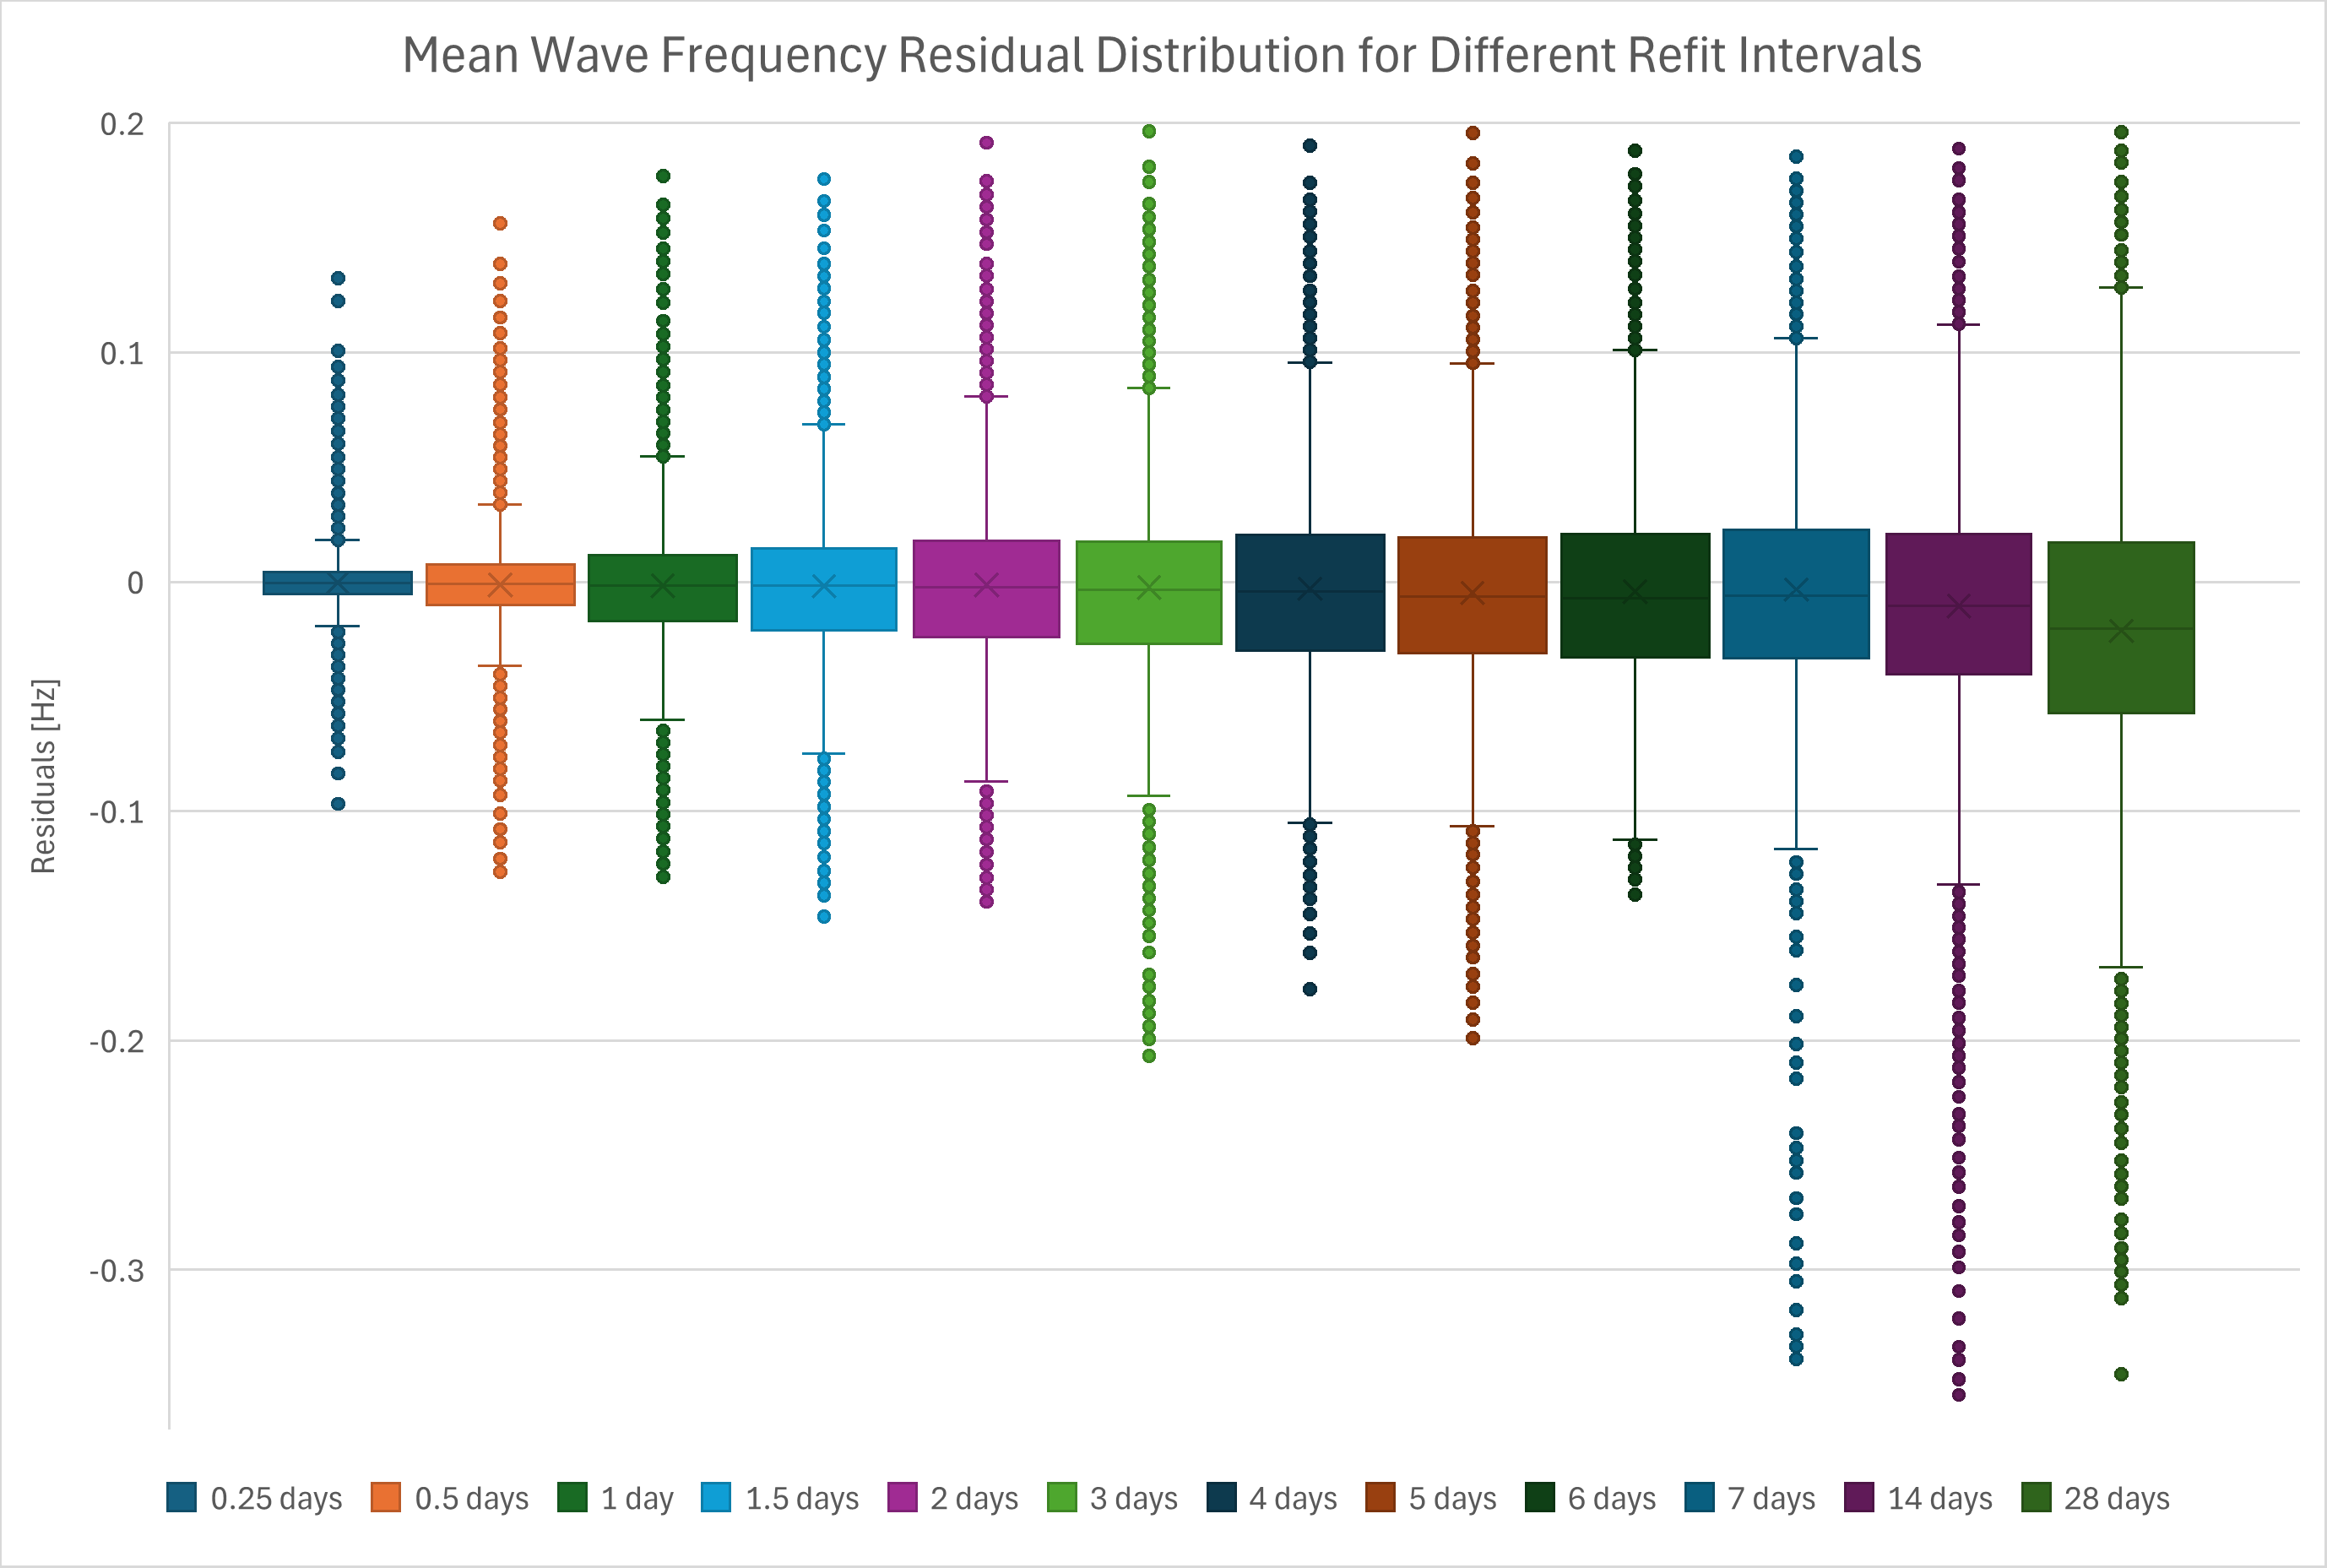
\includegraphics[width=\textwidth]{graphs/Box_refit_meanfr.png}
        \caption{Mean Wave Frequency}
        \label{fig:mean_fr_refit_box}
    \end{subfigure}
    \vskip\baselineskip
    \begin{subfigure}[b]{0.49\textwidth}
        \centering
        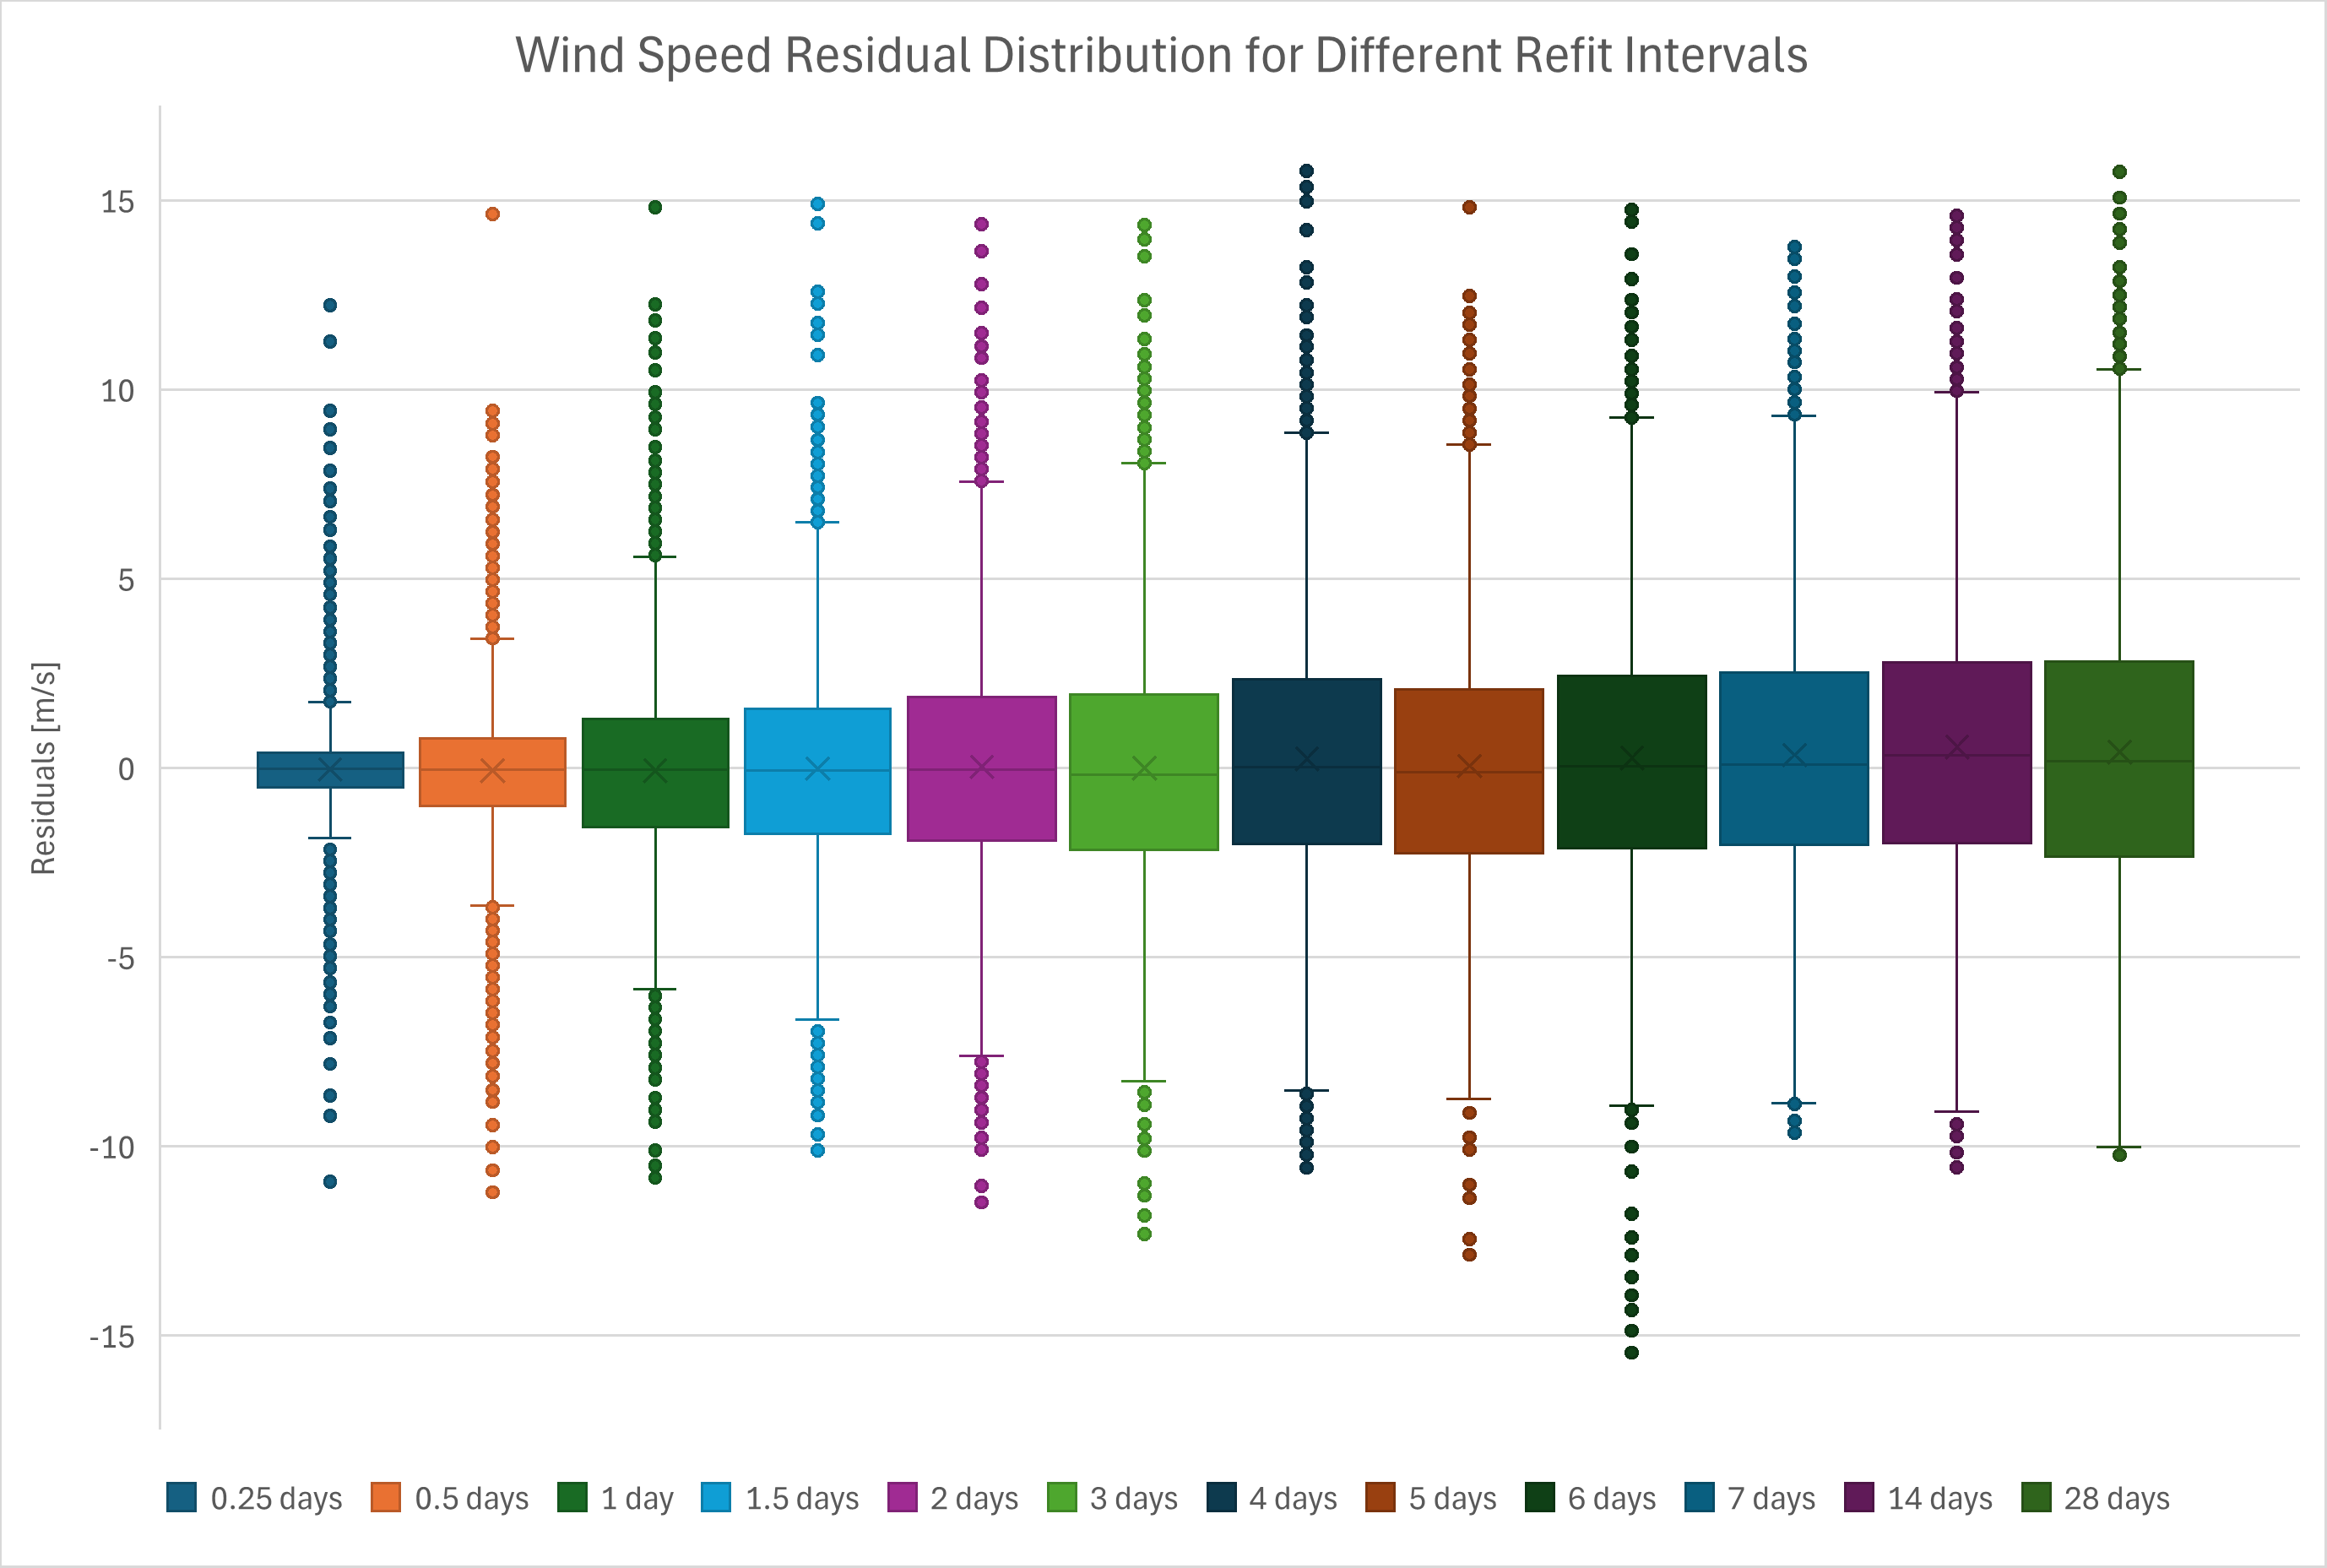
\includegraphics[width=\textwidth]{graphs/Box_refit_windspeed.png}
        \caption{Wind Speed}
        \label{fig:wind_speed_refit_box}
    \end{subfigure}
    \caption{Residual distribution of the Hybrid ARIMA–ANN model’s under varying refit intervals.}
    \label{fig:hybrid_refit_box}
\end{figure}

\newpage

\section{Implementation of Hybrid Model in Offshore Wind Turbine Installation}
\label{implementation_results}
From the operational limitations of the vessels for the mean wave frequency, from Table \ref{table:operational_limits}, it is seen that the mean wave frequency has a limit of 9 seconds and 7 seconds for respectively a Crane Barge and a Heavy Lift Vessel. Comparing this to the actual mean wave frequency in 2009, Figure \ref{fig:jack-up vessel usage}. It can be seen that in almost every case the mean wave frequency goes over the operational limit of both these vehicles. In practice, this means the installation will be done with a Jack-Up vessel.\\

\begin{figure}[ht!]
    \centering
    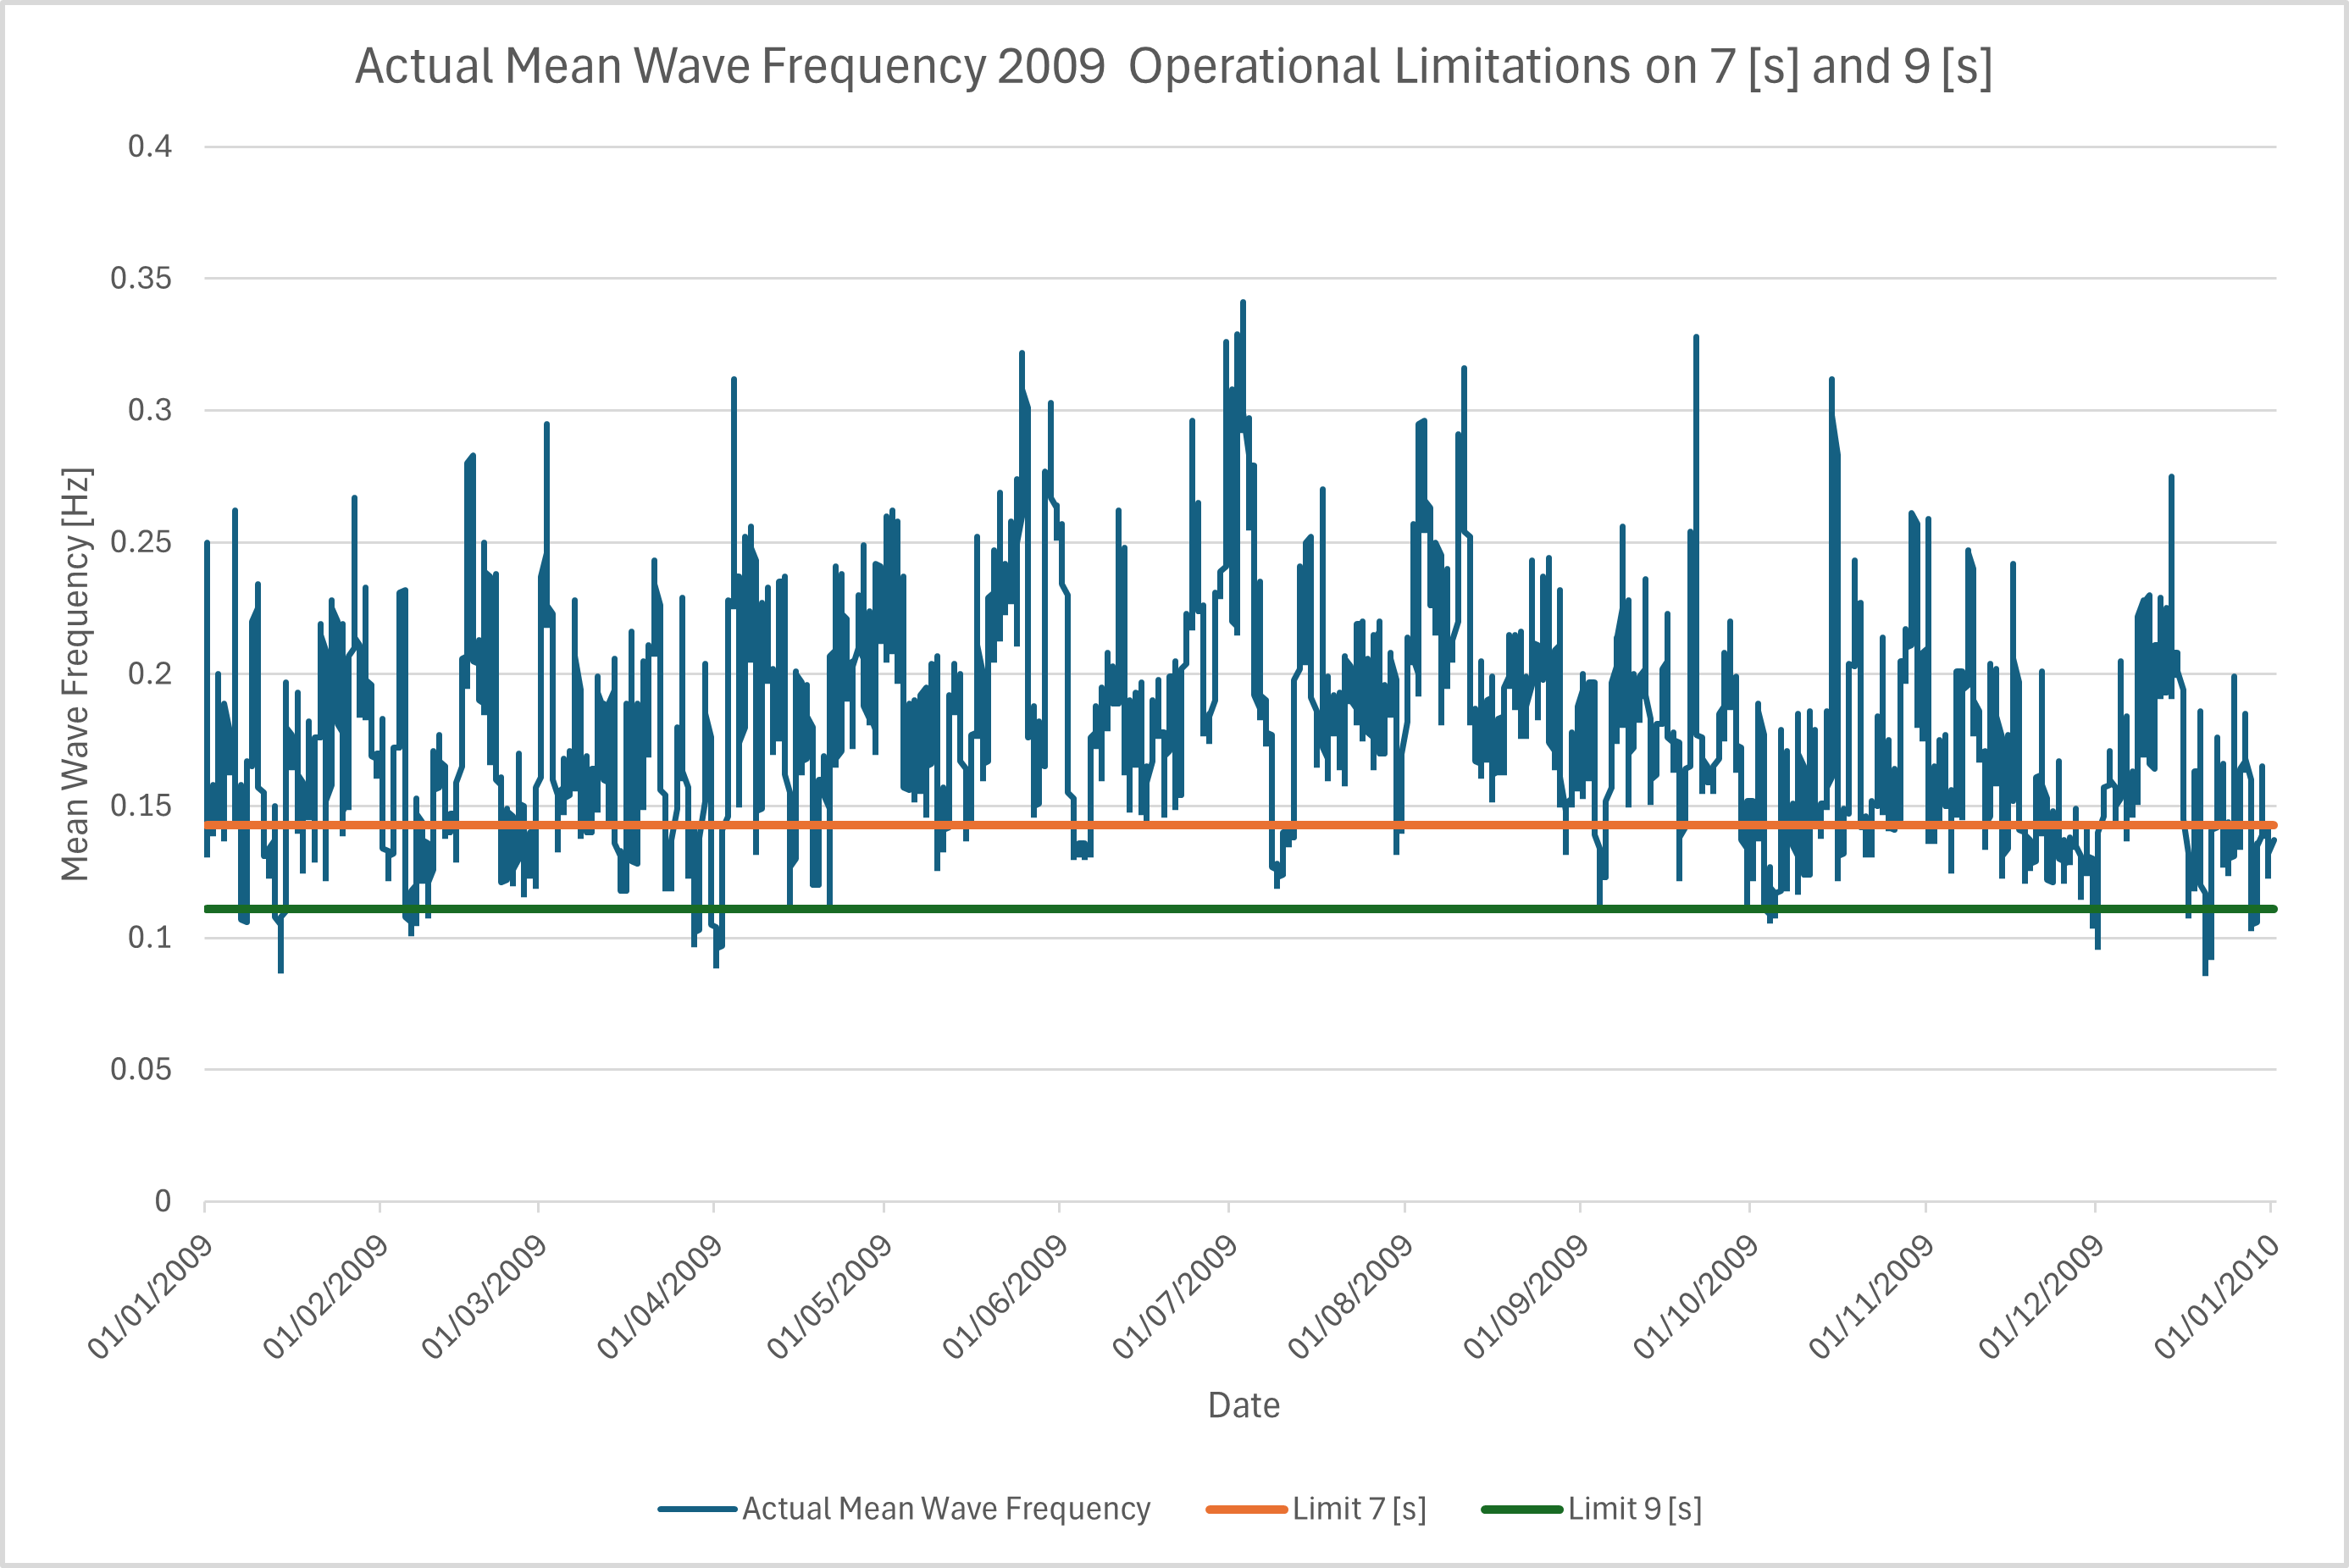
\includegraphics[width=0.6\linewidth]{graphs/Limitation on usage other ships then jack-up vessel.png}
    \caption{Operational limit for mean wave frequency of 7 and 9 [s]}
    \label{fig:jack-up vessel usage}
\end{figure}

\noindent The Operational Limitations of the Jack-Up Vessel from Table \ref{table:operational_limits} are re-shown below in Table \ref{table:operational_limits_jackup}. It follows that the Mean Wave Frequency does not influence the operational limits, so this will not be further investigated, the focus will be on the significant wave height and the wind speed. With their operational limitations, the actual outcomes of the Hybrid model are evaluated. A confusion matrix is constructed for both parameters and both limitations, with this the influence of different refit intervals is shown in Tables \ref{tab:swh_confusion_derived}, \ref{tab:wind_speed_8}, \ref{tab:wind_speed_10} and \ref{tab:wind_speed_16}.\\


\begin{table}[ht!]
    \centering
    \caption{Operational Limits for Key Weather Conditions During Installation Phases (Jack-Up Vessel)}
    \label{table:operational_limits_jackup}
    \begin{tabular}{|l|c|c|}
        \hline
        \textbf{Phase} & \textbf{Significant Wave Height} & \textbf{Wind Speed} \\
        \hline
        Monopile         & 2.5 & 16 \\
        \hline
        Transition Piece & 2.5 & 16 \\
        \hline
        Tower            & 2.5 & 10 \\
        \hline
        Nacelle          & 2.5 & 10 \\
        \hline
        Blade            & 2.5 & 8 \\
        \hline
    \end{tabular}
\end{table}

\noindent The confusion matrices below show the True Positive (TP), True Negatives (TN), False Positives (FP) and False Negatives (FN) for the model concerning the actual values. A TP occurs when the actual model and the forecast model both show a value above the limit, a TN when both are below. A FP when the forecast thinks the operational limit has been reached, but in practice this is not the case. FN is the most concerning, while the forecast thinks the operation could be done but the actual values are too high, which will lead to unsafe conditions. In the same manner FP would lead to stoppage of the installation, while unnecessary, and the costs associated with down-time. To further investigate these matrices, a False Positive Rate, a False Negative Rate and the Accuracy are calculated with the Formulas \ref{eq:fprate}, \ref{eqfnr} and \ref{eq:accuracy}.\\

\begin{equation}
\label{eq:fprate}
\text{FP Rate} = \frac{\text{False Positive}}{\text{False Positive} + \text{True Negative}}
\end{equation}

\begin{equation}
\label{eqfnr}
\text{FN Rate} = \frac{\text{False Negative}}{\text{False Negative} + \text{True Positive}}
\end{equation}

\begin{equation}
\label{eq:accuracy}
\text{Accuracy} = \frac{\text{True Positive} + \text{True Negative}}{\text{Total Observations}}
\end{equation}

\begin{table}[ht!]
    \centering
    \caption{Confusion Matrix and Derived Metrics for Significant Wave Height 2.5 m Operational Limit}
    \label{tab:swh_confusion_derived}
    \begin{tabular}{|l|c|c|c|c|c|c|c|c|}
        \hline
        \textbf{Refit Interval} & \textbf{TP} & \textbf{TN} & \textbf{FP} & \textbf{FN} && \textbf{FP Rate} & \textbf{FN Rate} & \textbf{Accuracy} \\
        \hline
        0.25 days & 2296 & 14661 & 232  & 331  && 1.56\%  & 12.60\% & 96.79\% \\
        0.5 days  & 2011 & 14462 & 431  & 616  && 2.89\%  & 23.45\% & 94.02\% \\
        1 day     & 1476 & 14135 & 758  & 1151 && 5.09\%  & 43.81\% & 89.10\% \\
        1.5 days  & 1139 & 14136 & 757  & 1488 && 5.08\%  & 56.64\% & 87.19\% \\
        2 days    & 882  & 14019 & 874  & 1745 && 5.87\%  & 66.43\% & 85.05\% \\
        3 days    & 570  & 13865 & 1028 & 2057 && 6.90\%  & 78.30\% & 82.39\% \\
        4 days    & 490  & 14074 & 819  & 2137 && 5.50\%  & 81.35\% & 83.13\% \\
        5 days    & 683  & 13677 & 1216 & 1944 && 8.16\%  & 74.00\% & 81.96\% \\
        6 days    & 429  & 13501 & 1392 & 2198 && 9.35\%  & 83.67\% & 79.51\% \\
        7 days    & 533  & 13841 & 1052 & 2094 && 7.06\%  & 79.71\% & 82.04\% \\
        14 days   & 701  & 13503 & 1390 & 1926 && 9.33\%  & 73.32\% & 81.07\% \\
        28 days   & 435  & 12360 & 2533 & 2192 && 17.01\% & 83.44\% & 73.03\% \\
        \hline
    \end{tabular}
\end{table}

\begin{table}[ht!]
    \centering
    \caption{Confusion Matrix and Derived Metrics for Wind Speed 8 m/s Operational Limit}
    \label{tab:wind_speed_8}
    \begin{tabular}{|l|c|c|c|c|c|c|c|c|}
        \hline
        \textbf{Refit Interval} & \textbf{TP} & \textbf{TN} & \textbf{FP} & \textbf{FN} && \textbf{FP Rate} & \textbf{FN Rate} & \textbf{Accuracy} \\
        \hline
        0.25 days & 6669 & 9374 & 686  & 791  && 6.82\%  & 10.60\% & 91.57\% \\
        0.5 days  & 5989 & 8923 & 1137 & 1471 && 11.30\% & 19.72\% & 85.11\% \\
        1 day     & 5137 & 8069 & 1991 & 2323 && 19.79\% & 31.14\% & 75.38\% \\
        1.5 days  & 4467 & 7636 & 2424 & 2993 && 24.10\% & 40.12\% & 69.08\% \\
        2 days    & 3866 & 7540 & 2520 & 3594 && 25.05\% & 48.18\% & 65.10\% \\
        3 days    & 3679 & 7224 & 2836 & 3781 && 28.19\% & 50.68\% & 62.23\% \\
        4 days    & 2739 & 7649 & 2411 & 4721 && 23.97\% & 63.28\% & 59.29\% \\
        5 days    & 3212 & 7224 & 2836 & 4248 && 28.19\% & 56.94\% & 59.57\% \\
        6 days    & 2730 & 7426 & 2634 & 4730 && 26.18\% & 63.40\% & 57.97\% \\
        7 days    & 2381 & 7625 & 2435 & 5079 && 24.20\% & 68.08\% & 57.11\% \\
        14 days   & 1977 & 7763 & 2297 & 5483 && 22.83\% & 73.50\% & 55.59\% \\
        28 days   & 1768 & 7837 & 2223 & 5692 && 22.10\% & 76.30\% & 54.82\% \\
        \hline
    \end{tabular}
\end{table}

\begin{table}[ht!]
    \centering
    \caption{Confusion Matrix and Derived Metrics for Wind Speed 10 m/s Operational Limit}
    \label{tab:wind_speed_10}
    \begin{tabular}{|l|c|c|c|c|c|c|c|c|}
        \hline
        \textbf{Refit Interval} & \textbf{TP} & \textbf{TN} & \textbf{FP} & \textbf{FN} && \textbf{FP Rate} & \textbf{FN Rate} & \textbf{Accuracy} \\
        \hline
        0.25 days & 3489 & 12959 & 417  & 655  && 3.12\%  & 15.81\% & 93.88\% \\
        0.5 days  & 2982 & 12719 & 657  & 1162 && 4.91\%  & 28.04\% & 89.62\% \\
        1 day     & 2098 & 12521 & 855  & 2046 && 6.39\%  & 49.37\% & 83.44\% \\
        1.5 days  & 1621 & 12601 & 775  & 2523 && 5.79\%  & 60.88\% & 81.18\% \\
        2 days    & 1194 & 12616 & 760  & 2950 && 5.68\%  & 71.19\% & 78.82\% \\
        3 days    & 924  & 12442 & 934  & 3220 && 6.98\%  & 77.70\% & 76.29\% \\
        4 days    & 557  & 12653 & 723  & 3587 && 5.41\%  & 86.56\% & 75.40\% \\
        5 days    & 848  & 12718 & 658  & 3296 && 4.92\%  & 79.54\% & 77.43\% \\
        6 days    & 642  & 12563 & 813  & 3502 && 6.08\%  & 84.51\% & 75.37\% \\
        7 days    & 552  & 12755 & 621  & 3592 && 4.64\%  & 86.68\% & 75.95\% \\
        14 days   & 369  & 12813 & 563  & 3775 && 4.21\%  & 91.10\% & 75.24\% \\
        28 days   & 482  & 12215 & 1161 & 3662 && 8.68\%  & 88.37\% & 72.47\% \\
        \hline
    \end{tabular}
\end{table}

\begin{table}[ht!]
    \centering
    \caption{Confusion Matrix and Derived Metrics for Wind Speed 16 m/s Operational Limit}
    \label{tab:wind_speed_16}
    \begin{tabular}{|l|c|c|c|c|c|c|c|c|}
        \hline
        \textbf{Refit Interval} & \textbf{TP} & \textbf{TN} & \textbf{FP} & \textbf{FN} && \textbf{FP Rate} & \textbf{FN Rate} & \textbf{Accuracy} \\
        \hline
        0.25 days & 127 & 17245 & 24  & 124 && 0.14\%  & 49.40\% & 99.16\% \\
        0.5 days  & 77  & 17231 & 38  & 174 && 0.22\%  & 69.32\% & 98.79\% \\
        1 day     & 46  & 17262 & 7   & 205 && 0.04\%  & 81.67\% & 98.79\% \\
        1.5 days  & 23  & 17262 & 7   & 228 && 0.04\%  & 90.84\% & 98.66\% \\
        2 days    & 28  & 17256 & 13  & 223 && 0.08\%  & 88.84\% & 98.65\% \\
        3 days    & 13  & 17269 & 0   & 238 && 0.00\%  & 94.82\% & 98.64\% \\
        4 days    & 24  & 17264 & 5   & 227 && 0.03\%  & 90.44\% & 98.68\% \\
        5 days    & 8   & 17266 & 3   & 243 && 0.02\%  & 96.81\% & 98.60\% \\
        6 days    & 14  & 17232 & 37  & 237 && 0.21\%  & 94.42\% & 98.44\% \\
        7 days    & 3   & 17269 & 0   & 248 && 0.00\%  & 98.80\% & 98.58\% \\
        14 days   & 0   & 17269 & 0   & 251 && 0.00\%  & 100.00\% & 98.57\% \\
        28 days   & 0   & 17269 & 0   & 251 && 0.00\%  & 100.00\% & 98.57\% \\
        \hline
    \end{tabular}
\end{table}

\noindent For the significant wave height in Table \ref{tab:swh_confusion_derived} it can be seen that the change between a 7-day refit interval and a 14-day refit interval does not influence the accuracy by a lot. Where there is a slight decrease in the accuracy, the large forecast window of 14 days would mean operations could be planned much longer in advance. In most cases, however, the significant wave height does not exceed the operational limit, as can be seen in the low amount of TP and FN values.\\

\noindent For Table \ref{tab:wind_speed_16} the operational limit is too high, which shows a model that is almost perfect in capturing it. For Tables \ref{tab:wind_speed_8} and \ref{tab:wind_speed_10} the relevance of accurate forecasting is evident. Especially for a wind speed of 8 [m/s], looking at the longer refit intervals in almost 50 \% of the cases the model fails to capture the limit correctly. With a high percentage of FN, but still a fairly low percentage for FP, the model. The same can be seen in Table \ref{tab:wind_speed_10} where more values are below the operational limit and so the model performs overall better.  